\documentclass[a4paper,openright,twoside,12pt]{book}
\usepackage[a4paper,left=4cm,right=2cm,top=3cm,bottom=3cm]{geometry}
\usepackage[spanish]{babel}
\usepackage[latin1]{inputenc}
\usepackage[T1]{fontenc}
\usepackage{lmodern}
\usepackage{mathtools}
\usepackage{amsmath}
\usepackage{amssymb}
\usepackage{gensymb} % simbolo de grado (\degree)
\usepackage{graphicx}
\usepackage{subcaption} 
\usepackage{mathrsfs} %% simbolos de transformadas de fourier
\usepackage[font=small]{caption}
\usepackage[sort&compress]{natbib} %% Para comprimir las cites
\usepackage{setspace} %% cambiar interlineado
\interfootnotelinepenalty=10000 % saco el limite de las footnote a 1 linea por pagina

%% ---------------
%% | NEWCOMMANDS |
%% ---------------
\newcommand{\promedio}[1]{\langle #1 \rangle}
\newcommand{\paginavacia}{\newpage \thispagestyle{empty} $\ $}
%% Elimino numero de pagina y header de pagina anterior a capitulo:
%% (es para usar con openright y hay que ponerlo antes de cada capitulo, excepto el primero)
\newcommand{\prechapterpage}{
	\ifthenelse{\isodd{\thepage}}{
	\newpage
        %~ \phantom{placeholder} % doesn't appear on page
        $\ $
	\thispagestyle{empty} % if want no header/footer
	\newpage
	}{}
}
%% Agregar paginas en blanco manteniendo apertura a izquierda (para usar con openany)
\usepackage{ifthen}
\newcommand{\prepartpage}{
	\ifthenelse{\isodd{\thepage}}{\newpage}{
	\newpage
        %~ \phantom{placeholder} % doesn't appear on page
        $\ $
	\thispagestyle{empty} % if want no header/footer
	\newpage
	}
}


%% DEFINO CARPETAS
\newcommand{\Simbolos}{./Simbolos}
\newcommand{\Tapa}{./Tapa}
\newcommand{\Introduccion}{./Introduccion}
\newcommand{\ConceptosGeofisica}{./ConceptosGeofisica}
\newcommand{\Curie}{./Curie}
\newcommand{\Flexion}{./Flexion}
\newcommand{\Conclusiones}{./Conclusiones}

%% -----------------------------------------------------------------------------------


\begin{document}

 

\begin{titlepage}


\newgeometry{left=2cm, right=1cm, top=1.5cm, bottom=1.5cm}
\centering

\begin{minipage}[c]{0.16\textwidth}
\centering
\includegraphics[width=0.85\textwidth]{\Tapa/figs/unr.jpg}    
\end{minipage}
\begin{minipage}[c]{0.65\textwidth}
\centering{}
{\scshape \small
Departamento de F�sica\\
Escuela de Ciencias Exactas y Naturales\\
Facultad de Ciencias Exactas, Ingenier�a y Agrimensura\\
Universidad Nacional de Rosario\\
}
\end{minipage}
\begin{minipage}[c]{0.16\textwidth}
\centering
\includegraphics[width=1\textwidth]{\Tapa/figs/fceia.jpg}    
\end{minipage}


\vspace*{1.8cm}
\centering

{\large \bf TESINA DE GRADO PARA OPTAR POR\\}
{\large \bf EL T�TULO DE LICENCIADO EN F�SICA\\}

\vspace*{1\baselineskip} % White space at the top of the page


\begin{minipage}[c]{0.9\textwidth}
    \centering
    
    \rule{\textwidth}{1.6pt}\vspace*{-\baselineskip}\vspace*{2pt} % Thick horizontal line
    \rule{\textwidth}{0.4pt}\\[\baselineskip] % Thin horizontal line
    
    \begin{spacing}{2.0}
    {\huge \bf  M�todos Espectrales para la Determinaci�n de la Profundidad del Punto de Curie y el Espesor El�stico de la Corteza Terrestre}\\[0.2\baselineskip] % Title
    \end{spacing}
    
    \rule{\textwidth}{0.4pt}\vspace*{-\baselineskip}\vspace{3.2pt} % Thin horizontal line
    \rule{\textwidth}{1.6pt}\\[\baselineskip] % Thick horizontal line
\end{minipage}

\centering
{\scshape % Texto en mat�sculas con primera letra grande y el resto m�s chicas

\vspace{0.5cm}

Autor\\
{\Large Santiago Rub�n Soler \par} % Editor list
\vspace{0.5cm}

Director\\
{\Large Dr. Mario E. Gim�nez \par} % Editor list

\vspace{0.5cm}

Consejero de Estudios\\
{\Large Dr. Pablo A. Turner \par} % Editor list
}




\vfill



\includegraphics[width=0.14\textwidth]{\Tapa/figs/igsv.png}

\vspace{0.1cm}
{\scshape \small En colaboraci�n con el \\ \small Instituto Geof�sico-Sismol�gico Ing. Volponi \\ \small Universidad Nacional de San Juan}

\vspace{0.5cm}
{\scshape \large 2015}

\restoregeometry
\end{titlepage}





\prepartpage
\pagenumbering{roman}
\setcounter{page}{3}
\pagestyle{plain}
\tableofcontents{}



\vspace*{0.4cm}
{\bf \huge Lista de S�mbolos}
\addcontentsline{toc}{part}{Lista de S�mbolos}
\vspace*{0.8cm}

\renewcommand{\arraystretch}{1.5}

\begin{tabular}{c l}
$\phi$: & Latitud \\
$\lambda$: & Longitud \\
$G$: & Constante de Gravitaci�n Universal (6.67384e-11 m/s$^{2}$) \\
$g$: & Aceleraci�n de la gravedad normal \\
$\Delta g_{fa}$: & Anomal�a de Aire Libre \\
$\Delta g_{bg}$: & Anomal�a de Bouguer \\
$\Delta T$: & Anomal�a Magn�tica \\
mGal: & Unidad de aceleraci�n, equivalente a 10$^{-5}$m/s$^{2}$ \\
TF: & Transformada de Fourier \\
FFT: & Transformada R�pida de Fourier (Fast Fourier Transform) \\
$\Phi_{\Delta T} \left( {\bf k} \right)$: & Espectro de Potencias de la Anomal�a Magn�tica $\Delta T$ \\
$\overline{\Phi}_{\Delta T}$(k): & Promedio Radial de $\Phi_{\Delta T} \left( {\bf k} \right)$ \\
${\bf k}$: & Vector de frecuencias \\
$t$: & Ancho de la corteza normal \\
$h$: & Altura topogr�fica \\
$w$: & Deflexi�n de la Ra�z \\
$\rho_{t}$: & Densidad de la Topograf�a \\
$\rho_{c}$: & Densidad de la Corteza \\
$\rho_{m}$: & Densidad del Manto \\
$T_{e}$: & Espesor El�stico \\
$D$: & Rigidez Flexural \\
$Z_{t}$: & Profundidad al techo de la loza magnetizada\\
$Z_{c}$: & Profundidad al centroide de la loza magnetizada\\
$Z_{b}$: & Profundidad al piso de la loza magnetizada \\
\end{tabular}


\prepartpage{}
%~ \paginavacia{}

%~ \pagestyle{plain}
%~ \chapter*{Introducci�n}\addcontentsline{toc}{part}{Introducci�n}


\vspace*{0.4cm}
{\bf \huge Introducci�n}
\addcontentsline{toc}{part}{Introducci�n}

\vspace*{0.8cm}

La Geof�sica es la rama de la ciencia que posee como objeto de estudio el Planeta Tierra desde un punto de vista f�sico, concentrada en los procesos y propiedades f�sicas del mismo. Su objetivo es ahondar en la comprensi�n de su estructura, evoluci�n y los fen�menos que en �l se generan. El origen de estas inquietudes acerca de nuestro planeta data de tiempos ancestrales. Los primeros pensadores ya intentaban dar explicaciones a los fen�menos naturales que los rodeaban, mientras que en ciertas civilizaciones ya hac�an uso de herramientas como la br�jula o instrumentos s�smicos, de los cuales se sabe de su existencia desde el a�o 132 AC. El auge del pensamiento cient�fico tampoco fue indiferente a esta rama del conocimiento: luego de formular sus Teor�as sobre Mec�nica, Newton las aplic� para el estudio de la precesi�n del equinoccio, entre otros.

Sin embargo, la Geof�sica no fue considerada una disciplina independiente hasta el siglo XIX. A partir de entonces los avances tecnol�gicos acompa�aron el crecimiento de esta ciencia, posibilitando la aparici�n de nuevos y mejores instrumentos de medici�n (desde magnet�metros prot�nicos hasta mediciones via sat�lites) como tambi�n de nuevas herramientas computacionales que permiten acelerar el an�lisis de cada vez mayores cantidades de datos.

En este trabajo haremos foco en la modelizaci�n de la �ltima capa de la Tierra que se conoce como Lit�sfera, compuesta por la corteza terrestre y el manto superior. A�n contando con los avances tecnol�gicos nombrados en el p�rrafo anterior, la adquisici�n de datos por perforaci�n contin�a siendo poco accesible, dificultosa y s�lo nos brinda informaci�n de los primeros metros de la corteza. Es por ello que es necesario recurrir a m�todos indirectos que nos den informaci�n de la Lit�sfera a partir de datos que podamos obtener en la superficie terrestre o en altura. Estos m�todos est�n basados en la modelizaci�n f�sica de la Lit�sfera.

A lo largo de este trabajo propondremos dos m�todos fundados en otros ya existentes: uno que parte del an�lisis del magnetismo para la Determinaci�n de la Profundidad al Punto de Curie, y otro que utiliza datos gravim�tricos y cartas de topograf�a para la Determinaci�n del Espesor El�stico de la Corteza Terrestre. Adem�s, expondremos los programas computaciones que se implementaron con fin de aplicar estas metodolog�as, mostrando en ambos casos, sus funcionamientos sobre modelos sint�ticos as� como tambi�n sobre una zona actualmente bajo estudio: la cuenca Neuquina. Si bien el objetivo principal del trabajo no es la interpretaci�n y entendimiento de dicha zona, decidimos aportar a su estudio desde los m�todos aqu� implementados.

El punto en com�n que poseen ambos es que la resoluci�n de los modelos se realizan en el espacio de frecuencia, es por ello que podemos introducirlos dentro de la categor�a de m�todos espectrales; los cuales han tenido su auge en muchas �reas cient�ficas y tecnol�gicas, as� como tambi�n dentro de la Geof�sica, con la aparici�n del m�todo de las Transforamdas R�pidas de Fourier, a mediados de los a�os 60'. A trav�s de este algoritmo optimizado es posible trasladar los problemas hacia el espacio de frecuencias muy r�pidamente, reduciendo los tiempos de c�lculo.

Los programas computaciones para aplicar algunas de las metodolog�as ya existentes se distribuyen bajo licencias privativas. Frente a esto, es nuestro deseo que las implementaciones de los m�todos que aqu� propondremos se encuentren bajo licencias de Software Libre, con el fin de que todos puedan beneficiarse con ellos y que tengan la libertad de estudiarlos, modificarlos y distribuirlos si as� lo desean.

Para realizar esta tarea elegimos utilizar el lenguaje de programaci�n Python. La principal raz�n de esta elecci�n reside en que tanto el int�rprete como la mayor parte de las librer�as que posee se encuentran bajo Licencias de Software Libre. En segundo lugar, porque nos permite escribir c�digo de forma muy r�pida y entendible, liberando m�s cantidad de tiempo para trabajar sobre la idea que queremos implementar y haciendo m�s hincapi� en ella que en la construcci�n del c�digo. En tercer y �ltimo lugar lo elegimos debido a la existencia de poderosas librer�as cient�ficas y de c�lculo num�rico (SciPy y NumPy, \cite{SciPy}) como de ploteo (Matplotlib, \cite{Matplotlib}). Adem�s, durante el desarrollo del trabajo supimos de la existencia de una librer�a orientada a la aplicaci�n de m�todos Geof�sicos conocida como Fatiando a Terra (\cite{Uieda2014}), tambi�n bajo Licencias de Software Libre.


\vspace{0.5cm}

Como ya hemos dicho, en el desarrollo de este trabajo haremos foco en la modelizaci�n de la Lit�sfera. Es de especial inter�s entender su comportamiento tect�nico, composici�n y estructura debido a los fen�menos naturales que en ella ocurren (vulcanismo, sismicidad, orog�nesis, etc) y por la cantidad de recursos naturales que alberga.

Existe una superficie, a la cual haremos referencia frecuentemente, conocida como discontinuidad de Mohorovi\~ci\'c, tambi�n llamada Moho. Se trata de la superficie que delimita la corteza terrestre del manto superior. En oc�ano, la corteza normal suele tener un promedio de 6km de profundidad, mientras que para regiones continentales promedia los 35km. La presencia de cuerpos an�malos puede generar variaciones de esos valores, modificando la profundidad del Moho punto a punto. La Determinaci�n del Espesor El�stico de la corteza juega un papel importante en la forma en la cual la presencia de topograf�a en regiones continentales produce tal perturbaci�n en el Moho.

Tambi�n es necesario definir un marco de referencia para los datos con los cuales trabajaremos. Debido a la geometr�a regular que presenta la superficie terrestre, se hace muy dif�cil hallar una expresi�n matem�tica que la represente. Es por ello que es necesario definir una superficie que reproduzca ciertas caracter�sticas de la misma.

Desde un punto de vista geom�trico podemos realizar una primera aproximaci�n de la Tierra por una esfera cuyo radio es el radio promedio de la misma. Siendo este modelo muy rudimentario e insuficiente, podemos extender dicha aproximaci�n a un esferoide de revoluci�n que llamaremos Elipsoide de Referencia. 

En el presente trabajo se utiliz� el Elipsoide de Referencia WGS84 (World Geodetic System 1984), cuyo semieje mayor posee una longitud de $a = 6378137.0$ m y la inversa del achatamiento $1/f = 298.257 223 563$, de donde se obtiene un semieje menor de $b \simeq 6356752.314245$ m. Este representa un sistema de referencia est�ndar para datos de altitud y de geoide (vease secci�n \ref{section-geoide}), en coordenadas elipsoidales de latitud ($\phi$), longitud ($\lambda$) y altitud ($h$), donde $h(\lambda, \phi)=0$ reproduce el Elipsoide en cuesti�n.

Es com�n hallar los datos de muchas magnitudes referenciados en coordenadas elipsoidales, o tambi�n conocidas como geogr�ficas. Sin embargo, en determinadas ocasiones es necesario contar con informaci�n acerca de la distancia entre los puntos donde estos fueron tomados. Si la zona de estudio no es muy grande (no se extiende m�s a all� de algunos grados) es posible realizar una proyecci�n de los mismos a coordenadas planas cuyos ejes se encuentran en metros. A lo largo de este trabajo utilizaremos un tipo particular de proyecci�n, conocida como Gauss-Kr�ger. Se trata de un derivado de la Transversal de Mercator, y divide al territorio argentino entre distintas zonas o fajas longitudinales. Para realizarla haremos uso del software PROJ4, a trav�s de su interfaz en Python: pyproj.





\prepartpage{}
\pagenumbering{arabic}
\setcounter{page}{11}
\pagestyle{headings}
\part{Conceptos de F�sica y Geof�sica}


\chapter{Gravimetr�a e Isostasia}

Los m�todos gravim�tricos poseen un lugar formidable en la historia de la ciencia. Las primeras observaciones cuantificadas de la ca�da de los objetos tienen sus ra�ces en los experimentos de Galileo Galilei alrededor del a�o 1590. En 1687 Isaac Newton publica su famoso tratado {\it Philosophiae Naturalis Principia Mathematica} en el cual propone que la fuerza gravitatoria es una interacci�n entre toda la materia, incluido el planeta Tierra.

En 1672 un estudiante franc�s, Jean Richer, nota que un reloj pendular dise�ado para ser preciso en Par�s perd�a unos pocos minutos al d�a en Cayenne, Guinea Francesa. De esta forma se descubre que las observaciones con p�ndulos sirven para medir la variaci�n espacial del geopotencial gravitatorio. Newton interpret� correctamente esta diferencia entre ambas mediciones como consecuencia de la forma ``ovalada'' de la Tierra. Los franceses opinaban distinto, por lo que enviaron dos expediciones: una a las altas latitudes de Suecia y otra a Ecuador para medir cuidadosamente la longitud de un arco de un grado en ambos lugares para compararlos. La expedici�n a Ecuador estaba liderada por Pierre Bouguer, quien es conocido por la anomal�a que lleva su nombre.

La aplicaci�n de mediciones de gravedad a problemas geol�gicos se remonta a las hip�tesis rivales de John Pratt y George Airy publicadas entre 1855 y 1859 acerca del equilibrio isost�tico mediante el cual se soporta la topograf�a. En ese entonces notaron que las plomadas cerca del Himalaya se deflectaban de la vertical una cantidad menor de la predicha debido a la masa topogr�fica de la cadena monta�osa. Ambos propusieron que en la ausencia de fuerzas adem�s de la gravitatoria, las partes r�gidas de la corteza ``flotan'' en un substrato denso, por ende la masa total en cada columna vertical hasta la profundidad de compensaci�n debe equilibrarse punto a punto. De esa forma, las regiones elevadas deben estar compensadas por deficiencia de masa, mientras que las depresiones topogr�ficas est�n sustentadas por excesos de masas.

Pratt explic� estas observaciones en t�rminos de variaci�n lateral de la densidad, es decir, que los Himalayas estaban elevados por ser menos densos que la corteza que los rodea. Airy propuso encambio que la corteza posee una densidad uniforme, pero var�a su grosor, por ende la cadena monta�osa se eleva sobre el terreno que la rodea gracias a la presencia de ra�ces corticales.

\begin{flushright}
    \cite{Blakely1995}
\end{flushright}

\section{Potencial Gravitatorio y Geoide}\label{section-geoide}
Seg�n la Ley de Gravitaci�n Universal de Newton, el potencial gravitatorio generado por un diferencial de masa en un punto a una distancia $r$ del mismo es:

\begin{equation}
    dV = +G \frac{dm}{r} 
\end{equation}

donde G es la constante de gravitaci�n universal\footnote{Obs�rvese que se utiliza la convenci�n del signo positivo para la definici�n del potencial.}. Por ende, el potencial generado por una distribuci�n de masas con densidad $\rho(\vec{r})$ y volumen V puede escribirse como:
\begin{equation}
    W_{a}(\vec{r}) = G \int\limits_{V}  \frac{\rho(\vec{r}\,')}{|\vec{r} - \vec{r}\,'|} d\vec{r}\,'
\end{equation}

Puede demostrarse que este potencial satisface la ecuaci�n de Poisson:
\begin{equation}
    \nabla^{2} W_{a} = -4\pi G \rho
\end{equation}

Fuera de las masas la densidad $\rho$ se anula y el potencial satisface la ecuaci�n de Laplace:
\begin{equation}
    \nabla^{2} W_{a} = 0
\end{equation}
y por ende, $W_{a}$ es una funci�n harm�nica.

En el caso de que el cuerpo que genera dicho potencial sea la Tierra, no debemos dejar de considerar el efecto de rotaci�n de la misma, el cual genera un potencial centr�fugo $\Phi$.{}
\begin{equation}
    \Phi(\vec{r}) = \frac{1}{2} \omega^{2} d_{z}^{2}
\end{equation}
donde $\omega$ es la velocidad angular de la Tierra y $d_{z} = \sqrt{x^{2} + y^{2}}$ la distancia del punto $\vec{r}$ al eje rotacional ($z$).

En conclusi�n, el potencial gravitatorio generado por la Tierra fuera de sus masas puede escribirse como la suma de un potencial harm�nico y un potencial centr�fugo.
\begin{equation}
    W = W_{a} + \Phi
\end{equation}

Sin embargo, podemos replantear dicho potencial como la suma de dos potenciales: uno que llamaremos ``normal'' $U$ y otro denominado ``perturbativo'' $T$. Definiremos al primero de forma tal  que la superficie equipotencial dada por $U(\vec{r}) = U_{0}$ tenga la misma forma que el Elipsoide de revoluci�n. Mientras que el segundo ser� el potencial perturbador necesario para alcanzar el potencial $W$.

Reescribiendo los potenciales en las coordenadas elipsoidales $(h, \lambda, \phi)$, y teniendo en cuenta que $U$ no depende de $\lambda$, podemos expresar a $W$ como:
\begin{equation}
    W(h, \lambda, \phi) = U(h, \phi) + T(h, \lambda, \phi)
\end{equation}

Finalmente, definiremos al geoide como aquella superficie equipotencial definida por $W(h, \lambda, \phi) = U_{0}$ y ondulaci�n del geoide a la funci�n $N(\lambda, \phi)$ tal que:
\begin{equation}
    W(h \! = \! N(\lambda, \phi), \, \lambda, \, \phi) = U(h\!=\!0, \phi) = U_{0}
\end{equation}


%% METER FIGURA DE ELIPSOIDE GEOIDE Y ONDULACION DEL GEOIDE

\section{Anomal�as Gravim�tricas}

\subsection{Gravedad Normal y Anomal�a Gravim�trica}
Antes de poder hacer referencia a una anomal�a gravim�trica es necesario definir el escenario ``normal'' del cual dicha anomal�a se aparta. Para ello se utiliza el concepto de gravedad normal.

El vector de aceleraci�n de la gravedad puede obtenerse a partir del potencial que lo genera. Por ejemplo, el vector de gravedad generado por el potencial terrestre $W$ puede obtenerse de la siguiente manera\footnote{Obs�rvese que se utiliza la convenci�n del signo positivo para la definici�n del gradiente del potencial.}:
\begin{equation}
    \vec{g} = + \nabla W
\end{equation}

Y de aqu� obtenemos la componente radial de la aceleraci�n:
\begin{equation}
    g_{z} = \frac{\partial W}{\partial r}
\end{equation}

Ahora, podemos definir la gravedad normal como la componente radial del gradiente normal $U$ evaluada en la superficie del Elipsoide.
\begin{equation}
    g_{0} = \frac{\partial U}{\partial r} \Big|_{h=0}
\end{equation}

Aprovechando que el potencial $U$ es harm�nico, es posible realizar un desarrollo en harm�nicos esf�ricos y luego obtener el valor de $g_{0}$ como funci�n de $\phi$. Para el Elipsoide WGS84 $g_{0}$ adopta el siguiente:
\begin{equation}
    g_{0}(\phi) = 9.7803267714 \frac{1+0.00193185138639 \sin^2(\phi)}{\sqrt{1-0.00669437999013 \sin^2(\phi)}}
\end{equation}

Finalmente, podemos definir la anomal�a gravitatoria observada como la diferencia entre la gravedad observada y la normal:
\begin{equation}
    \Delta g(h, \lambda, \phi) = g_{z}(h, \lambda, \phi) - g_{0}(\phi)
\end{equation}


En la Figura \ref{fig-anomalias-1-2} se expone un ejemplo simple de un modelo de lit�sfera que incluye el manto, la corteza, una dada topograf�a junto con  la ra�z que genera, e incluye un cuerpo an�malo inmerso en corteza. En la primer gr�fica podemos apreciar la gravedad observada, es decir, la que genera el modelo completo junto con el resto de la Tierra. Mientras que en la segunda gr�fica se muestra c�mo se ve modificada al quitarle a dicha magnitud la gravedad normal. El efecto que posee esto sobre el modelo es el de remover la corteza normal y el manto, dejando una ra�z con un contraste de densidad negativo y parte del cuerpo an�malo con contraste de densidad positivo.

\subsection{Anomal�a de Aire Libre}


%% Arreglar esto!

Observemos que la anomal�a de gravedad observada posee una dependencia en $h$. Por ejemplo, si la medici�n fue realizada en topograf�a, $h$ vendr� a tomar el valor de la cota topogr�fica. Dicha dependencia resulta innecesaria, por lo cual es beneficioso eliminarla. Para realizarlo haremos uso de lo que se conoce como correcci�n de Aire Libre.

Esta consiste en quitar el efecto que produce el potencial normal $U$ al elevar el punto de medici�n desde el geoide a la altura $h$. El mismo se obtiene realizando una aproximaci�n por series de Taylor de la aceleraci�n de la gravedad:
\begin{equation}
    g(h) \simeq g_{0} + \frac{\partial g(h)}{\partial r} \, h \simeq g_{0} - 0.3086 \cdot 10^{-5} \, h
\end{equation}
donde la constante 0.3086 est� expresada en $s^{-2}$.

Definimos entonces el t�rmino de correcci�n de Aire Libre como:
\begin{equation}
    g_{fa}(h) = - 0.3086 \cdot 10^{-5} \, h
\end{equation}

Y la anomal�a de Aire Libre no ser� m�s que la Anomal�a de Gravedad Observada menos dicha correcci�n:
\begin{equation}
    \Delta g_{fa} = g_{z} - g_{0} - g_{fa}
\end{equation}

\begin{figure}[b!]
\centering
\includegraphics[width=0.98\textwidth]{\ConceptosGeofisica/figs/anomalias-fig-1-2.pdf}
\caption{Gravedad Observada y Anomal�a Observada para un ejemplo con Topograf�a, Ra�z y cuerpo an�malo en corteza, medidas en topograf�a.}
\label{fig-anomalias-1-2}
\end{figure}




\subsection{Anomal�a de Bouguer}
Adem�s de la correcci�n de Aire Libre, suele realizarse tambi�n otra correcci�n para eliminar el efecto que produce la topograf�a sobre dicha anomal�a. �sta se conoce como anomal�a de Bouguer.

La forma simple de la anomal�a de Bouguer consiste en aproximar la altura topogr�fica en un punto dado por un cilindro infinito y restarle el efecto que este genera a la anomal�a de Aire Libre en el mismo punto.
\begin{equation}
    g_{bg} = 2\pi g_{0} \rho_{c} h \simeq 0.1119 \cdot 10^{-5} \, h
\end{equation}
donde $\rho_{c} = 2670$ kg/m$^{3}$ es la densidad est�ndar de las masas topogr�ficas y la constante de proporcionalidad est� expresada en s$^{-2}$.

Finalmente, definimos la Anomal�a de Bouguer como:
\begin{equation}
    \Delta g_{bg} = \Delta g_{fa} - g_{bg} = g_{z} - g_{0} - g_{fa} - g_{bg}
\end{equation}


En la Figura \ref{fig-anomalias-3-4} se exponen las anomal�as de Aire Libre y de Bouguer para el mismo ejemplo que el de la Figura \ref{fig-anomalias-1-2}. En la primer gr�fica vemos que la correcci�n de Aire Libre quita el efecto que produce el haber obtenido las mediciones en altura, sin embargo no produce ninguna modificaci�n al modelo. Mientras que en la segunda gr�fica observamos c�mo la correcci�n de Bouguer elimina el efecto gravim�trico que produce la topograf�a.

\begin{figure}[b!]
\centering
\includegraphics[width=0.98\textwidth]{\ConceptosGeofisica/figs/anomalias-fig-3-4.pdf}
\caption{Anomal�a de Aire Libre y Anomal�a Simple de Bouguer para el mismo ejemplo que el de la Figura \ref{fig-anomalias-1-2}.}
\label{fig-anomalias-3-4}
\end{figure}

\section{Isostasia}
%%�Qu� es la isostasia? Watts
%% de Wikipedia:
La isostasia es el estado de equilibrio entre la corteza y el manto terrestre debido, entre otros factores, a la diferencia de densidades entre ambos. La corteza terrestre es generalmente menos densa que el manto, con lo cual, debido al principio de Arqu�medes, se puede interpretar que la primera flota sobre el segundo.

\subsection{Isostasia de Airy}
Existe un modelo isost�tico cl�sico conocido como Modelo Isost�tico de Airy-Heiskanen o Isostasia de Airy el cual predice que una elevaci�n topogr�fica produce una ra�z que se introduce en el manto a una profundidad que depende de dicha elevaci�n. El equilibrio se produce con la competencia de la fuerza gravitatoria de la corteza y el empuje generado por la diferencia de densidades del manto y la ra�z.

Dada una topograf�a arbitraria consideremos una columna de toda la lit�sfera (desde la topograf�a hasta el manto superior), como se puede apreciar en la Figura \ref{fig-airy}. Seg�n el modelo de Airy, el peso de la parte cortical de la columna (primer miembro de la ecuaci�n \ref{eq-airy-peso-empuje}) debe anularse con el empuje generado por el desplazamiento de manto debido a la intrusi�n de la ra�z (segundo miembro de la ecuaci�n \ref{eq-airy-peso-empuje}).
\begin{equation}
    \rho_{t}\,g\,h + \rho_{c}\,t\,g + \rho_{c}\,w\,g = \rho_{m}\,w\,g + \rho_{c}\,t\,g
    \label{eq-airy-peso-empuje}
\end{equation}

Reagrupando los t�rminos se obtiene la ecuaci�n de equilibrio isost�tico de Airy:
\begin{equation}
    w = \frac{\rho_{t}}{\rho_{m}-\rho_{c}} \, h
    \label{eq-airy}
\end{equation}

Al aplicar dicha ecuaci�n a cada punto del perfil o grilla es posible obtener la ra�z isost�tica. Como observaci�n, tomando valores normales de densidades de topograf�a, corteza y manto ($\rho_{t}=2670$ kg/m$^{3}$, $\rho_{t}=2900$ kg/m$^{3}$, $\rho_{m}=3300$ kg/m$^{3}$) la relaci�n de proporcionalidad entre la intrusi�n de la corteza en manto y la topograf�a queda:
\begin{equation}
    w \simeq 6,675 \, h
\end{equation}

\begin{figure}[h!]
\centering
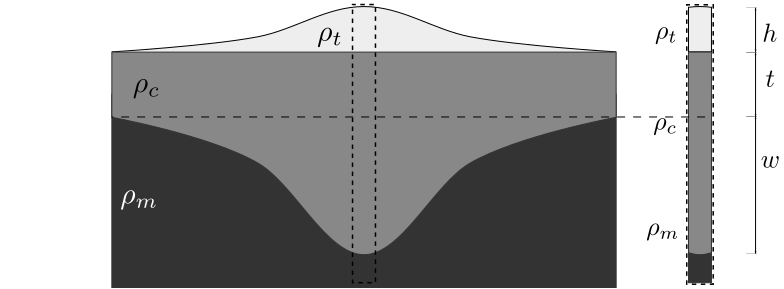
\includegraphics[width=0.75\textwidth]{\ConceptosGeofisica/figs/airy.pdf}
\caption{Perfil de lit�sfera con topograf�a, corteza normal, ra�z isost�tica de Airy y manto superior. En la columna elegida la topograf�a posee una altura $h$ y la ra�z una profundidad $w$ medida desde el limite inferior de la corteza normal, definida con un ancho $t$.}
\label{fig-airy}
\end{figure}



\prechapterpage
\chapter{Magnetometr�a y Magnetismo}
El campo geomagn�tico debe ser la propiedad geof�sica de la Tierra m�s ancestralmente estudiada. La atracci�n mutua entre imanes se remonta a los tiempos de Tales de Mileto, mientras que la tendencia de estas rocas a alinearse en direcciones preferenciales ya se conoc�an en China para el I D.C.

En el siglo XIII, Petrus Peregrinus llev� a cabo importantes experimentos con esferas de rocas magn�ticas, describiendo por primera vez los conceptos de polarizaci�n magn�tica, meridianos magn�ticos y la idea de que polos opuestos se atraen y polos iguales se repelen. En 1600, el f�sico William Gilbert public� su tratado {\it De Magnete} en el cual proclama que {\it ``la Tierra es un gran im�n''}, atribuy�ndole as� otra propiedad adem�s de la redondez al planeta Tierra. En 1838, el matem�tico Carl Friederich Gauss le otorg� a las mediciones geomagn�ticas el primer formalismo a escala global, aplicando el an�lisis de arm�nicos esf�ricos a un conjunto de mediciones disponibles en ese tiempo.

La aplicaci�n de m�todos magn�ticos a problemas geol�gicos avanz� en paralelo con el desarrollo de los magnet�metros. En 1630 se usaron br�julas para realizar prospecciones de oro en Suecia. Y Max Thomas Edelmann utiliz� magnetos balanceados en las primeras mediciones aeromagn�ticas en la primer d�cada del siglo pasado, los cuales permiten una mejor cobertura que las realizadas en tierra.

En 1955 Varian Associates dise�aron un magnet�metro prot�nico, un instrumento simple que mide la magnitiud total del campo magn�tico sin necesidad de estabilizadores o equipos de orientaci�n, el cual revolucion� las mediciones a�reas y terrestres, siendo el est�ndar en campa�as actuales.

Mientras que el campo gravitatorio es invariante en el tiempo, a excepci�n de algunos cambios por la redistribuciones de masas (como las mareas, movimientos magm�ticos, etc), el campo magn�tico terrestre var�a en intensidad y orientaci�n en escalas de tiempos que van desde los milisegundos a milenios. Esto hace parecer que la reducci�n de mediciones magn�ticas para el estudio de cuerpos de la corteza sea muy complicada, sin embargo en la pr�ctica no lo es.

Para poder alcanzar dicha reducci�n es necesario discriminar entre los campos magn�ticos generados por los cuerpos de la corteza y los originados por distintas otras fuentes, como el movimiento de magma en el interior de la Tierra, vientos solares, la presencia de la ion�sfera, etc.


\begin{flushright}
    \cite{Blakely1995}
\end{flushright}

\section{Potencial Magn�tico Terrestre}
En la mayor�a de las situaciones geof�sicas, las corrientes el�ctricas son despreciables en regiones donde se realizan las mediciones de magnetometr�a, por lo cual es posible expresar al campo magn�tico como el gradiente de un potencial escalar (caso contrario deber�amos hacer uso del potencial vector $\bf{A}$).
\begin{equation}
    \nabla \times {\bf B} = 0 \,\,\,\,\,\, \Rightarrow \,\,\,\,\,\, {\bf B} = - \nabla \varphi
\end{equation}

Adem�s, si consideramos una esfera de radio $a$ que no es atravesada por fuentes magn�ticas entonces el potencial $\varphi$ satisface la ecuaci�n de Laplace.
\begin{equation}
    \nabla^{2} \varphi = 0
\end{equation}

Si existen fuentes dentro y fuera de la esfera, entonces el potencial en las regiones libres de ellas y cercanas a su superficie, puede ser escrito como suma de los potenciales originados por fuentes internas ($i$) y externas ($e$) a la esfera, respectivamente.
\begin{equation}
    \varphi = a \sum\limits_{n=0}^{\infty} \left[ \left( \frac{r}{a} \right)^{n} T_{n}^{\,e} + \left( \frac{a}{r} \right)^{n+1} T_{n}^{\,i} \right]
\end{equation}
\begin{align}
    T_{n}^{i} &= \sum_{m=0}^{n} (g_{n}^{mi} \cos m\lambda  + h_{n}^{mi} \sin m\lambda ) P_{n}^{m}(\theta) \\
    T_{n}^{e} &= \sum_{m=0}^{n} (g_{n}^{me} \cos m\lambda  + h_{n}^{me} \sin m\lambda ) P_{n}^{m}(\theta)
\end{align}


Donde el �ngulo $\theta$ es la colatitud, es decir, 90$\degree$ - $\phi$, y $\lambda$ la longitud; las constantes $g_{n}^{m}$ y $h_{n}^{m}$ se conocen como coeficientes de Gauss; y $P_{n}^{m}$ es el polinomio asociado de Legendre de grado $n$ y orden $m$ normalizado seg�n la convenci�n de Schmidt \cite[p. 113]{Blakely1995}.

A partir de mediciones de campo magn�tico alrededor del globo es posible demostrar que las constantes $g_{n}^{me}$ y $h_{n}^{me}$ pueden ser despreciadas en una primera aproximaci�n, es decir, el campo magn�tico terrestre est� principalmente originado por las fuentes internas. Por simplicidad nos desharemos de los �ndices $i$ y $e$, y daremos por supuesto que las constantes $g_{n}^{m}$ y $h_{n}^{m}$ se refieren a fuentes internas. Sin embargo, se suele aplicar correcciones, como la diurna, para eliminar los efectos de las fuentes externas.

En conclusi�n, podemos escribir el potencial generado por fuentes internas a la Tierra como:
\begin{equation}
    \varphi = a \sum\limits_{n=1}^{\infty} \left( \frac{a}{r} \right)^{n+1} \sum\limits_{m=0}^{n} (g_{n}^{m} \cos m\lambda + h_{n}^{m} \sin m\lambda) P_{n}^{m}(\theta)
\end{equation}

Al igual que hicimos en gravimetr�a al introducir el Elipsoide, es necesario definir un marco de referencia para la magnetometr�a. Dicho sistema de referencia se construye al igual que el Elipsoide, por acuerdo internacional, y se lo denomina IGRF (International Geomagnetic Reference Field).

El IGRF consiste en establecer los t�rminos de Gauss hasta orden 10, ya que se ha demostrado que el campo generado por ellos representa en gran medida el campo originado en el n�cleo de la Tierra. Debido a sus variaciones temporales, se adopta un nuevo modelo IGRF cada 5 a�os, per�odo denominado {\it �poca}.

Es posible separar el potencial $\varphi$ entre dos componentes:
\begin{equation}
    \varphi = \varphi^{D} + \varphi^{ND} \\
\end{equation}
\begin{equation}
    \varphi^{D} = \frac{a^{3}}{r^{2}} \left[ g_{1}^{0}\frac{z}{r} + g_{1}^{1}\frac{x}{r} + h_{1}^{1}\frac{y}{r} \right]
\end{equation}

\begin{equation}
\left\{
\begin{aligned}
    x &= r \cos\lambda \, \sin\theta \\
    y &= r \sin\lambda \, \sin\theta \\
    z &= r \cos\theta
\end{aligned}
\right.
\end{equation}


La componente $\varphi^{D}$ coincide con el potencial generado por un dipolo magn�tico con magnetizaci�n ${\bf m} = \frac{4\pi}{\mu_{0}}a^{3}(g_{1}^{1}, \, h_{1}^{1}, \, g_{1}^{0})$ y se conoce como potencial dipolar, mientras que $\varphi^{ND}$ se denomina potencial no dipolar. Se puede demostrar que $\varphi^{ND}$ compone solo un 10$\%$ del campo total, por lo cual podemos considerar al campo magn�tico terrestre como dipolar a una muy buena aproximaci�n.

\section{Elementos del Campo Geomagn�tico}
A la hora de determinar el campo magn�tico terrestre en un dado punto de la superficie terrestre es posible hacerlo mediante sus tres componentes: $B_{x}$, $B_{y}$, $B_{z}$. De forma alternativa, es posible describirlo a partir de la intensidad total del campo $T$, y dos �ngulos: la inclinaci�n $I$ y la declinaci�n $D$.
\begin{gather}
    T = \sqrt{B_{x}^{2} + B_{y}^{2} + B_{z}^{2}} \\
    I = \arctan \frac{B_{z}}{\sqrt{B_{x}^{2} + B_{y}^{2}}} \\
    D = \arcsin \frac{B_{y}}{\sqrt{B_{x}^{2} + B_{y}^{2}}}
\end{gather}

\begin{figure}[t]
\centering
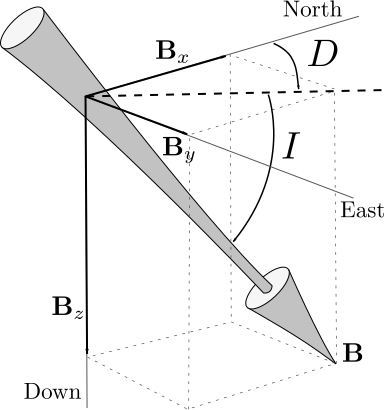
\includegraphics[width=0.35\textwidth]{\ConceptosGeofisica/figs/inclination-declination.pdf}
\caption{Ejemplo gr�fico de c�mo determinar los �ngulos de inclinaci�n $I$ y declinaci�n $D$ a partir del vector campo magn�tico $B$.}
\label{fig-inclination-declination}
\end{figure}

Dado un campo magn�tico ${\bf B}$, podemos ver en la Figura \ref{fig-inclination-declination} c�mo quedan definidos los �ngulos $I$ y $D$.

\section{Anomal�as Magn�ticas}
En los vuelos aeromagn�ticos se suelen utilizar magnet�metros escalares ({\it total-field magnetometers}) los cuales son capaces de medir la magnitud del campo magn�tico, sin importar la direcci�n del mismo.

La anomal�a magn�tica se define entonces como la diferencia entre la intensidad medida y la magnitud de un campo regional como puede ser el IGRF apropiado para el momento en el cual se llev� a cabo la medici�n. Si ${\bf T}$ representa el campo total en cualquier punto y ${\bf F}$ es el campo regional, entonces podemos escribir la anomal�a magn�tica como:
\begin{equation}
    \Delta T = |{\bf T}| - |{\bf F}|
\end{equation}

Adem�s de quitarle el campo generado por el IGRF, se suele realizar correcciones para extraer  las contribuciones de los fuentes externas. Un ejemplo de ellas es la correcci�n diurna, que elimina las contribuciones al campo magn�tico generado por la actividad solar.

\section[Transici�n de Fase Ferromagn�tica y Profundidad de Curie]{Transici�n de Fase Ferromagn�tica y \\Profundidad de Curie}
\chaptermark{Ferromagnetismo y Profundidad de Curie}

En p�rrafos anteriores hemos hecho menci�n sobre el origen del magnetismo terrestre en dos fuentes principales, una de ellas el n�cleo (especialmente el n�cleo exterior) y la otra, la corteza terrestre. La raz�n por la cual se descarta al manto como generador del campo geomagn�tico se debe a una caracter�stica de los materiales ferromagn�ticos como es la Temperatura de Curie.

Los materiales paramagn�ticos son aquellos que al estar expuestos a un campo magn�tico generan una magnetizaci�n en la misma direcci�n del campo, sin embargo, cuando el campo se desvanece, su magnetizaci�n vuelve a ser nula.

Por otro lado, los materiales ferromagn�ticos son aquellos que se comportan similar a los paramagnetos frente a un campo externo, sin embargo cuando este se anula, el material presenta una magnetizaci�n remanente no nula.

Sin embargo, los materiales ferromagn�ticos poseen dicha cualidad por debajo de una temperatura caracter�stica conocida como Temperatura de Curie. Una vez que la alcanzan sufren una Transici�n de Fase y se transforman en paramagnetos, es decir, no presentan m�s magnetizaciones remanentes.

En el interior de la Tierra las temperaturas aumentan con la profundidad, lo suficiente como para que dentro de la misma corteza superen la Temperatura de Curie de las rocas ferromagn�ticas all� presentes. A la profundidad en la cual las rocas sufren la transici�n de fase se la conoce como Profundidad al Punto de Curie, o Profundidad de Curie.

Por debajo de dicha profundidad podemos considerar que no existen fuentes de campo magn�tico, no hasta alcanzar el n�cleo externo, donde el campo magn�tico se genera por movimientos de fluidos, un mecanismo distinto al de magnetizaciones remanentes en la corteza.

De conocer la naturaleza de las rocas presentes en la corteza es posible determinar cu�l es la Temperatura de Curie de las mismas y por ende la Profundidad de Curie puede ser tomada como una isoterma, es decir, una superficie que posee la misma temperatura en todos sus puntos. Sin embargo hay que tener especial cuidado al realizar esto, ya que las Temperaturas de Curie de diversas rocas pueden variar hasta centenas de grados.


\prechapterpage
\chapter[M�todos Espectrales y FFT]{M�todos Espectrales y Transformada R�pida de Fourier}

Un camino posible para la interpretaci�n de anomal�as es trabajar con {\bf m�todos directos}, es decir, proponer un modelo inicial de los cuerpos causantes de dicha anomal�a construido a partir del conocimiento geol�gico y geof�sico ya existente de la zona de estudio, para luego ajustar par�metros para mejorar el ajuste de la anomal�a resultante con la observada.
Con modelo entendemos la distribuci�n geom�trica de cuerpos an�malos con par�metros caracter�sticos como densidad, susceptibilidad, resistencia, magnetizaci�n, etc.

La desventajas que presentan estos m�todos residen en en la necesidad de poseer informaci�n a priori sobre nuestra zona, lo cual no siempre es posible, y adem�s en un aspecto m�s intr�nseco del problema: la ambig�edad de la soluci�n. Est� demostrado que dado un potencial, ya sea gravitatorio o magn�tico, existen diversas distribuciones de densidades que generan el mismo resultado, un ejemplo de esto es la Capa Equivalente de Green \cite[p. 61]{Blakely1995}. Por lo tanto, si el conocimiento de la zona no es preciso, nuestra soluci�n al problema por estos m�todos puede llegar a ser err�nea, aunque los valores de anomal�as ajusten de forma excelente.
Por �ltimo, pero no menos importante, estos m�todos se llevan a cabo mediante prueba y error, lo cual resulta en un costo de tiempo y trabajo elevado hasta alcanzar la soluci�n.

Los m�todos opuestos a estos �ltimos son los llamados {\bf m�todos de inversi�n}, en los cuales la soluci�n al problema se obtiene de forma directa desde las anomal�as. Se propone un tipo de comportamiento de los cuerpos an�malos y se ajustan los par�metros seg�n dicho modelo. 
En este caso al modelo lo entendemos como la respuesta f�sica que genera cualquier distribuci�n arbitraria de los cuerpos an�malos que estamos considerando.

Los beneficios que otorgan estos m�todos est�n relacionados con el ahorro de trabajo, ya que la resoluci�n del problema puede ser encarada computacionalmente, como tambi�n generan m�s confiabilidad ya que necesitan menos informaci�n a priori. La desventaja que presentan reside en la falta de generalizaci�n, es decir, es posible que la zona de estudio no responda seg�n el modelo geof�sico propuesto, por lo cual el resultado que se obtenga de la inversi�n ser� err�neo.

Dentro de estos m�todos podemos ubicar a algunos {\bf m�todos espectrales}, como los que desarrollamos en este trabajo. Estos hacen uso de la Tansformada de Fourier para trasladar el problema hacia el espacio de frecuencias, donde algunos problemas como la continuaci�n ascendente \footnote{Continuaci�n Ascendente: es la obtenci�n de la anomal�a generada por cualquier distribuci�n \\ de densidades a una altura arbitraria conociendo �nicamente la anomal�a a una altura menor.} se reducen a relaciones lineales.

La Transformada de Fourier (TF) de cualquier funci�n $f(x)$ se puede definir de la siguiente manera:
\begin{equation}
    \mathcal{F} \left[ f(x) \right](k) = \int\limits_{-\infty}^{\infty} f(x) \, e^{-i k x} \, dx
\end{equation}
donde $k=2\pi/\lambda$ es el n�mero de onda y $\lambda$ es la longitud de onda asociada a $k$. Por conveniencia, hablaremos de forma indistinta del n�mero de onda y de la frecuencia haciendo referencia siempre al $k$, aunque se indique lo contrario.

Una de las propiedades importantes que posee la Transformada de Fourier es la identidad que relaciona la Transformada de una funci�n con la Transformada de su derivada n-�sima:
\begin{equation}
    \mathcal{F}[f^{(n)}(x)](k) = (ik)^{n} \,\, \mathcal{F}[f(x)](k)
    \label{eq-transformada-de-la-derivada}
\end{equation}

Adem�s, la Transformada de Fourier puede definirse para funciones de m�s de una variable, siendo el caso de inter�s para el presente trabajo, la Transformada de Fourier en 2D:
\begin{equation}
     \mathcal{F} \left[ f({\bf r}) \right]({\bf k}) = \int\limits_{-\infty}^{\infty} f({\bf r}) \, e^{-i {\bf k} \cdot {\bf r}} \, d{\bf r}
\end{equation}
donde ${\bf r} = (x, y)$ y ${\bf k}=(k_{x}, k_{y})$ ahora son vectores.

No fue hasta las d�cadas de los 60 y 70 que los m�todos espectrales comenzaron a tener mayor atenci�n para la resoluci�n de problemas geof�sicos. Este auge fue causado por el reciente desarrollo del algoritmo de \cite{Cooley1965} denominado Transformada R�pida de Fourier (FFT), el cual permite llevar a cabo la resoluci�n de una Transformada de Fourier Discreta (ecuaci�n \ref{eq-dft}) de forma muy eficiente, disminuyendo considerablemente los tiempos de c�lculo.
\begin{gather}
    F_{kl} =  \sum_{m=0}^{M-1} \sum_{n=0}^{N-1} f_{mn}\exp\left\{-2\pi i \left(\frac{mk}{ M}+\frac{nl}{N}\right)\right\} \quad k = 0, \ldots, M-1;\quad l = 0, \ldots, N-1 
    \label{eq-dft}
\end{gather}

Una desventaja de los m�todos espectrales es la necesidad de que los datos se encuentren ubicados en los nodos de una grilla regular, es decir, una cuadr�cula de puntos equiespaciados. En el caso de campa�as aeromagn�ticas esto no presenta un problema, ya que la densidad de puntos medidos es lo suficientemente alta como para que los algoritmos de interpolaci�n de los datos a los puntos de la grilla sea muy fiel al dato original.

Sin embargo existen situaciones donde los puntos no poseen tales caracter�sticas, sino que pueden describir caminos o regiones sin datos (algo que suele suceder en mediciones terrestres que pueden presentar obst�culos hacia determinadas zonas). En estos casos se debe tener precauci�n a la hora de interpretarlos, ya que los algoritmos de interpolaci�n pueden estar rellenando err�neamente esas regiones vac�as.

Otra caracter�stica contraproducente de las TF es que suelen producir efectos de borde, es decir, en los l�mites de la grilla los m�todos espectrales suelen cometer errores y no responder como lo hacen en los puntos m�s interiores. Esto se origina en la hip�tesis de que la funci�n $f$ debe ser peri�dica en todo el espacio $\Re^{2}$. Como no se poseen datos en todo ese espacio al trabajar con cantidades discretas, se transforma la funci�n $f$ en peri�dica extendi�ndola a infinito con un per�odo igual al ancho de la grilla. De esta forma solo se hace necesario calcular las componentes espectrales para longitudes de ondas menores a ese per�odo. Es por ello que es conveniente siempre disponer de datos en �reas mayores a la zona de estudio, para poder luego descartar los valores cercanos a los bordes.

Por �ltimo podemos notar que la Transformada de Fourier resulta ser una funci�n compleja en el espacio de frecuencias. En varios casos se suele hacer uso de lo que se conoce como el Espectro de Potencia de una funci�n $f(x,y)$, el cual se define como el cuadrado del m�dulo de la Transformada de Fourier de la funci�n $f$:
\begin{equation}
    \Phi_{f}({\bf k}) = \left| \, \mathcal{F}[f({\bf r})]\, \right|^{2}
\end{equation}


%%%% REVISAR BIEN EN BIBLIOGRAFIA
Una propiedad importante que posee el espectro de potencia es que si la funci�n $f$ posee �nicamente valores reales, entonces su Espectro de Potencia $\Phi_{f}({\bf k})$ ser� sim�trico con respecto al origen.


\prepartpage
%~ \newevenside
\part{Determinaci�n de la Profundidad del Punto de Curie}


%~ \newevenside
\chapter{Modelo de Loza Infinita}

La utilizaci�n de m�todos espectrales para la determinaci�n del Punto de Curie a partir de las anomal�as magn�ticas se originaron al poco tiempo de la divulgaci�n de la Transformada R�pida de Fourier. Estos podr�an clasificarse en dos tipos: aquellos que examinan el efecto de cuerpos an�malos aislados, y por otro lado los que examinan de forma estad�stica las propiedades de las anomal�as.

Uno de los trabajos pioneros del �ltimo grupo es el de \cite{Spector1970}, en el cual los autores presentan una forma compacta del espectro de potencial de un ensamble de prismas con magnetizaciones arbitrarias; aplicando los desarrollos de \cite{Bhattacharyya1964} para la determinaci�n de la anomal�a magn�tica generada por un prisma y el Principio Fundamental de la Mec�nica Estad�stica.

\cite{Blakely1995} condensa el modelo construido por \cite{Spector1970} de la siguiente manera: dada una loza con superficies superiores e inferiores a profundidades $Z_{t}$ y $Z_{b}$, respectivamente; extendida infinitamente en las direcciones horizontales, y con magnetizaci�n $M(x,y)$ arbitraria, el espectro de potencia de la anomal�a magn�tica medida que genera en $z=0$ puede escribirse como:
\begin{equation}
    \Phi_{\Delta T}({\bf k}) = \Phi_{M}({\bf k}) \,\, \Big\{ 4\pi^2 C_{m}^{2} |\Theta_{m}|^{2} |\Theta_{f}|^{2} \Big\}  \Big\{ e^{-2|{\bf k}|Z_{t}} \Big[ 1 - e^{-|{\bf k}|(Z_{b}-Z_{t})} \Big]^{2} \Big\}
\end{equation}
donde ${\bf k}$ es el n�mero de onda, $\Phi_{M}(k_{x},k_{y})$ es el espectro de potencia de la magnetizaci�n $M(x,y)$, $C_{m}$ es una constante de proporcionalidad y $\Theta_{m}$ y $\Theta_{f}$ son factores relacionados con la direcci�n de la magnetizaci�n y del campo geomagn�tico, respectivamente. Este modelo propone la existencia de un l�mite a una profundidad $Z_{b}$ a partir del cual no existen magnetizaciones. Se puede entender este l�mite como el Punto a la Profundidad de Curie, ya que m�s all� de eso las magnetizaciones remanentes son inexistentes.

Vale observar que todos los factores de la ecuaci�n anterior son radialmente sim�tricos, excepto por $\Phi_{\Delta M}(k_{x},k_{y})$, $|\Theta_{m}|^{2}$ y $|\Theta_{f}|^{2}$. Sin embargo, se puede demostrar que los promedios radiales de los �ltimos dos son constantes; por ende, el promedio radial del espectro de potencial puede ser escrito de la siguiente manera:
\begin{equation}
    \overline{\Phi}_{\Delta T} \,(k) = \promedio{\Phi_{\Delta T} \,(k)} = B \, \promedio{\Phi_{M}(k)} \,  e^{-2 k Z_{t}} \Big[ 1 - e^{-k(Z_{b}-Z_{t})} \Big]^{2}
\end{equation}
donde $k$ es el m�dulo de ${\bf k}$ y $B$ es una constante de proporcionalidad.

De conocer el comportamiento de la magnetizaci�n $M(x,y)$ en cada punto de la corteza, el c�lculo de su espectro radial es trivial y la determinaci�n de las profundidades de la loza 
son f�ciles de obtener. Sin embargo en situaciones geof�sicas eso no sucede, por lo cual debemos proponer un modelo estad�stico adecuado para $M(x,y)$.

A lo largo de la bibliograf�a el modelo de preferencia es proponer que $M(x,y)$ es completamente aleatoria y no correlacionada. En ese caso, el espectro de potencia de $M(x,y)$ es constante y la ecuaci�n anterior se reduce a:
\begin{equation}
    \overline{\Phi}_{\Delta T} \,(k) = A e^{-2 k Z_{t}} \Big[ 1 - e^{-k(Z_{b}-Z_{t})} \Big]^{2}
    \label{eq-blakely-espectro}
\end{equation}
donde $A$ es una nueva constante de proporcionalidad. Y finalmente, aplicando el logaritmo en ambos miembros obtenemos la siguiente expresi�n:

\begin{equation}
    \ln \overline{\Phi}_{\Delta T} \,(k) = \ln A - 2Z_{t}\, k + 2\, \ln \left( 1 - e^{-k(Z_{b}-Z_{t})} \right)
    \label{eq-blakely-ln-espectro}
\end{equation}

\begin{figure}[t!]
    \centering{}
    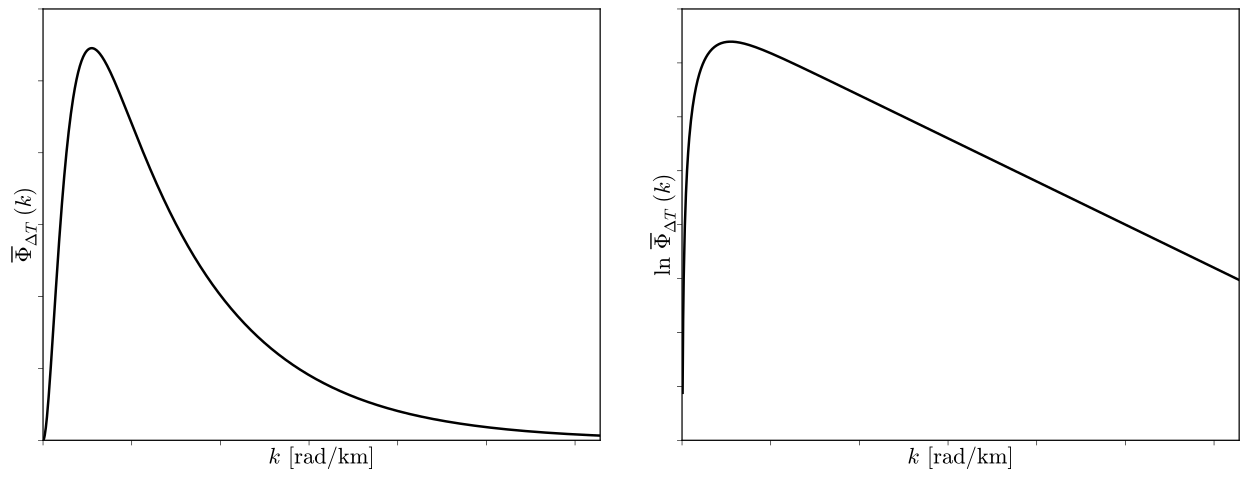
\includegraphics[width=0.98\textwidth]{\Curie/figs/blakely-espectros.pdf}
    \caption{Gr�ficas de promedios radiales del espectro de potencia de anomal�as magn�ticas y de su logaritmo, seg�n el modelo de \cite{Spector1970} y \cite{Blakely1995}.}
    \label{fig-blakely-espectros}
\end{figure}

En la Figura \ref{fig-blakely-espectros} se muestran las gr�ficas correspondientes a las ecuaciones anteriores (\ref{eq-blakely-espectro} y \ref{eq-blakely-ln-espectro}). Actualmente, las diversas metodolog�as existentes intentan ajustar los par�metros $Z_{b}$ y $Z_{t}$ a partir del espectro de potencias de las anomal�as magn�ticas.


\section{M�todos Actuales}

\cite{Tanaka1999} proponen realizar dos aproximaciones a la ecuaci�n \ref{eq-blakely-espectro}: una para baja frecuencias y otra para altas frecuencias (ecuaciones \ref{eq-tanaka-low-freq} y \ref{eq-tanaka-high-freq}, respectivamente).
\begin{align}
    \overline{\Phi}_{\Delta T}(k) \simeq 4 A (Z_{b}-Z_{c})^{2} \, k^{2} \, e^{-2 k Z_{t}} \quad &\Rightarrow \quad \ln \left[ \, \overline{\Phi}_{\Delta T}(k)^{1/2}/k \, \right] \simeq \ln C - Z_{c} \, k
    \label{eq-tanaka-low-freq} \\
    \overline{\Phi}_{\Delta T}(k) \simeq A \, e^{-2 k Z_{t}} \quad &\Rightarrow \quad \ln \left[ \, \overline{\Phi}_{\Delta T}(k)^{1/2} \, \right] \simeq \ln D - Z_{t} \, k
    \label{eq-tanaka-high-freq}
\end{align}

$C$ y $D$ son constantes y $Z_{c}$ es la profundidad del centroide de la loza ($2 Z_{c} = Z_{b} + Z_{t}$).

Ambas aproximaciones permiten relacionar linealmente funciones del espectro de potencia de las anomal�as con las profundidades del centroide y del techo de la loza. Esto reduce la obtenci�n de los par�metros a un simple ajuste lineal de los puntos (ver Figura \ref{fig-tanaka-graficas}). Una vez estimadas ambas cantidades es posible obtener el valor para el piso de la misma, es decir, la Profundidad de Curie.

\begin{figure}[t!]
\centering
\includegraphics[width=0.98\textwidth]{\Curie/figs/tanaka-graficas.png}
\caption{Aplicaci�n del m�todo propuesto por \cite{Tanaka1999} para el promedio radial de un espectro de potencia dado. Se muestran dos gr�ficas con las funciones necesarias para obtener las relaciones lineales expuestas en las ecuaciones \ref{eq-tanaka-low-freq} y \ref{eq-tanaka-high-freq} y sobre ellas los segmentos utilizados para el ajuste de las profundidades.}
\label{fig-tanaka-graficas}
\end{figure}

Este m�todo permite determinar la Profundidad de Curie en diversos puntos de nuestra zona de estudio, construyendo ventanas cuadradas de los datos de anomal�a magn�tica y realizando un c�lculo como el que se describi� en el p�rrafo anterior para cada uno de estos puntos.

Una de las desventajas que hallamos en este m�todo es la ausencia de herramientas que permitan discriminar si la ventana de datos de anomal�a que se utiliza es lo suficientemente ``buena'' como para llevar a cabo el ajuste de los par�metros.

Adem�s, encontramos que esta metodolog�a deja libre a nuestra subjetividad qu� puntos tomar para realizar el ajuste de las rectas. C�mo se pueden ver en la Figura \ref{fig-tanaka-graficas}, la determinaci�n de ambas pendientes puede verse modificada en funci�n de qu� puntos de las curvas tomamos para realizar el ajuste, conllevando una estimaci�n err�nea de los par�metros que deseamos precisar.

Una posible soluci�n a este problema es analizar cu�l es el rango de validez de cada aproximaci�n, con lo cual podr�amos identificar de forma m�s objetiva qu� puntos debemos seleccionar para realizar los ajustes por m�nimos cuadrados.

Por otro lado, \cite{Ross2006} proponen otro m�todo que soluciona algunos de los problemas mencionados. Su m�todo consiste en construir una ventana de datos de ancho $W$ por cada punto en donde desean determinar las profundidades $Z_{t}$ y $Z_{b}$ . Luego proceden a aumentar el tama�o de la ventana hasta que observan un pico en la gr�fica del $\ln \overline{\Phi}_{\Delta T} \,(k)$. La presencia del pico indica que las dimensiones de la ventana son suficientemente grandes como para incluir las bajas frecuencias asociadas al piso de la loza magn�tica.

Finalmente ajustan manualmente la curva de la ecuaci�n \ref{eq-blakely-ln-espectro} a los puntos de m�s baja frecuencia, ya que a partir de un determinado $k$ el scatter de puntos se desv�a de la recta te�rica, lo que podemos interpretar como la componente de ruido que poseen los datos de anomal�as magn�ticas.


\begin{figure}[t!]
\centering
\includegraphics[width=0.98\textwidth]{\Curie/figs/ross-graficas.png}
\caption{Ejemplo del m�todo de \cite{Ross2006} para la determinaci�n de la Profundidad de Curie. La gr�fica a) corresponde a una ventana de 130km de ancho, mientras que la b) a una de 180km. Las curvas negras corresponden a los datos, mientras que cada curva de color hace referencia a un ajuste con un par de par�metros distintos.}
\label{fig-ross-graficas}
\end{figure}

Este m�todo resuelve uno de los problemas de \cite{Tanaka1999}, dando un criterio para discriminar entre las ``buenas'' ventanas, de las que no lo son. Adem�s advierte que la mejor forma de elegir los puntos sobre los cuales estimar las profundidades no es construir una grilla de puntos como lo hace \cite{Tanaka1999}, sino elegirlos cuidadosamente, intentando que la ventana quede dentro de una ``regi�n magn�tica'', es decir que no posean informaci�n de lozas de diferentes profundidades.

Sin embargo, sigue incorporando un ingrediente subjetivo en el an�lisis, ya que el ajuste de la curva lo llevan a cabo de forma manual, a prueba y error, argumentando que sus ajustes por m�nimos cuadrados no respond�an a situaciones geof�sicamente posibles.


\section{�nalisis del Espectro de Potencia}
Partiendo de la ecuaci�n \ref{eq-blakely-espectro} podemos concluir sencillamente que los rangos de validez de las aproximaciones propuestas por \cite{Tanaka1999} en las ecuaciones \ref{eq-tanaka-low-freq} y \ref{eq-tanaka-high-freq} vienen dadas por las ecuaciones \ref{eq-tanaka-validez-low} y \ref{eq-tanaka-validez-high}, respectivamente.
\begin{align}
    k \ll 1/(Z_{b}-Z_{t})
    \label{eq-tanaka-validez-low} \\
    k \gg 1/(Z_{b}-Z_{t})
    \label{eq-tanaka-validez-high}
\end{align}

Al intentar utilizar estos rangos de validez nos encontramos con el problema de que ellos mismos est�n delimitados por los par�metros que deseamos calcular, por lo cual nos resultan poco �tiles.

\begin{figure}[t]
\centering
\includegraphics[width=0.98\textwidth]{\Curie/figs/tanaka-validez-5-35.pdf}
\caption{Promedio radial del espectro de potencias de las anomal�as magn�ticas (a) y su logaritmo (b), seg�n la ecuaci�n \ref{eq-blakely-espectro} junto con las curvas correspondientes a las aproximaciones de bajas y altas frecuencias para una loza de $Z_{t}=5\,{\rm km}$ y $Z_{b}=35\,{\rm km}$ ($Z_{c}=20\,{\rm km}$).}
\label{fig-tanaka-validez-5-35}
\end{figure}


\begin{figure}[t]
\centering
\includegraphics[width=0.98\textwidth]{\Curie/figs/tanaka-validez-18-22.pdf}
\caption{Promedio radial del espectro de potencias de las anomal�as magn�ticas (a) y su logaritmo (b), seg�n la ecuaci�n \ref{eq-blakely-espectro} junto con las curvas correspondientes a las aproximaciones de bajas y altas frecuencias para una loza de $Z_{t}=18\,{\rm km}$ y $Z_{b}=22\,{\rm km}$ ($Z_{c}=20\,{\rm km}$).}
\label{fig-tanaka-validez-18-22}
\end{figure}

Consideremos por ejemplo dos lozas: una gruesa de $Z_{t}=5\,{\rm km}$ y $Z_{b}=35\,{\rm km}$ y otra delgada de $Z_{t}=18\,{\rm km}$ y $Z_{b}=22\,{\rm km}$. En ambos casos, el centroide est� ubicado en $Z_{c}=20\,{\rm km}$. En las Figuras \ref{fig-tanaka-validez-5-35} y \ref{fig-tanaka-validez-18-22} se muestran los promedios radiales de los espectros de potencia y sus logaritmos junto con las gr�ficas correspondientes a las aproximaciones de bajas y altas frecuencias para la loza gruesa y delgada, respectivamente.

Como podemos apreciar en ellas, \cite{Ross2006} est�n en lo correcto al hacer hincapi� en la necesidad de observar el pico en las gr�ficas del $\ln \overline{\Phi}_{\Delta T} \,(k)$, ya que de otra forma no se obtiene informaci�n sobre el piso de la loza magn�tica. Es necesario tambi�n contar con informaci�n de frecuencias altas o intermedias. Esto en la pr�ctica se ve facilitado ya que si somos capcaes de observar las componentes de ruido, entonces podemos afirmar que alcanzamos frecuencias suficientemente altas.

En conclusi�n, una ventana satisfactoria para la obtenci�n de nuestras profundidades es aquella cuyo espectro de frecuencia exhibe un pico con buena resoluci�n y una recta hasta encontrarse con las frecuencias activadas por el ruido.
 
A�n as� vimos necesario realizar an�lisis cuantitativos sobre dicho espectro y la construcci�n de la ventana.


\subsection{Estimaci�n del Ancho de la Ventana}
Consideremos una ventana cuadrada de ancho $W$ y distancia entre primeros vecinos $d$ (distancia de sampleo). Derivando la ecuaci�n \ref{eq-blakely-espectro} ei igualando a cero, se obtiene la frecuencia $k_{p}$ en la cual se da el pico (ver Figura \ref{fig-espectro-blakely-anotaciones} a).

\begin{equation}
    \frac{\partial \, \overline{\Phi}_{\Delta T}}{\partial k}\Bigg|_{k_{p}} \!\!\!\!  =0 \quad \Rightarrow \quad   k_{p} = \frac{\ln(Z_{b})-\ln(Z_{t})}{Z_{b}-Z_{t}}
\end{equation}

Si definimos a $k_{0}$ la frecuencia fundamental ($k_{0}=2\pi / W$) y deseamos ubicar $(\alpha-1)$ puntos antes del pico, entonces $k_{0}$ debe ser:

\begin{equation}
    k_{0} = \frac{k_{p}}{\alpha}
\end{equation}

Podemos hallar una relaci�n entre el ancho de la ventana y las profundidades de la loza sustituyendo $k_{p}$ entre las ecuaciones anteriores.
\begin{equation}
    W = 2\pi \alpha \frac{Z_{b}-Z_{t}}{\ln(Z_{b})-\ln(Z_{t})}
\end{equation}

Con el fin de simplificar la dependencia del ancho de la ventana $W$ con respecto a las profundidades $Z_{b}$ y $Z_{t}$, definimos al cociente de estas dos como $\xi = Z_{b}/Z_{t}$. Reescribiendo la ecuaci�n anterior se obtiene:
\begin{equation}
    W = 2 \pi \alpha \, Z_{t} \, \frac{\xi-1}{\ln(\xi)}
    \label{eq-tamano-ventana}
\end{equation}

Si consideramos que $Z_{b}$ puede llegar a ser hasta diez veces mayor que $Z_{t}$ (lo cu�l es l�gico para una loza gruesa), entonces el factor dependiente de $\xi$ en la ecuaci�n \ref{eq-tamano-ventana} barre valores desde 1 a 4 para lozas delgadas a m�s gruesas, como se muestra en la Figura \ref{fig-grafica-xi}.

\begin{figure}[b!]
\centering
\includegraphics[width=0.7\textwidth]{\Curie/figs/xi.pdf}
\caption{Gr�fica del factor dependiente de $\xi=Z_{b}/Z_{t}$ de la ecuaci�n \ref{eq-tamano-ventana}.}
\label{fig-grafica-xi}
\end{figure}

\label{parrafo-ejemplo-curie}Por ejemplo, si queremos obtener 2 puntos entre $k=0$ y $k_{p}$ ($\alpha=3$) para una ventana con $Z_{b}=25{\rm km}$ y $Z_{t}=5{\rm km}$, es decir $\xi=5$, el tama�o de ventana que necesitamos es aproximadamente de $T=234{\rm km}$.


\subsection{Estimaci�n de la Distancia de Sampleo}

Como dijimos antes, en la pr�ctica resulta sencillo discernir si la distancia de sampleo que utilizamos es suficientemente peque�a analizando la presencia de ruido en nuestro espectro. Sin embargo, resulta interesante analizar qu� valor de $d$ deber�a ser suficientemente peque�o, ya que al subestimarlo se incrementa considerablemente la cantidad de puntos por ventana y con ello el tiempo de c�mputo de las Transformadas de Fourier.

Un criterio ser�a exigirle a nuestro espectro de potencias que el ancho del pico (aquel que aparece en la gr�fica del $\overline{\Phi}_{\Delta T}(k)$) ocupe una porci�n $1/\beta$ de todo el eje de frecuencias. Su ancho puede ser definido como la distancia entre $k=0$ y $\sigma_{k}$, siendo esta la frecuencia en la cual el espectro de potencia presenta el segundo punto de inflexi�n (v�ase Figura \ref{fig-espectro-blakely-anotaciones} a).

Para obtener el valor de $\sigma_{k}$ es necesario analizar cu�ndo se anula la derivada segunda del espectro de potencia. Dicha ecuaci�n no posee soluci�n anal�tica, sin embargo podemos obtener un valor aproximado calculando el punto de inflexi�n de la ra�z cuadrada del espectro de potencia: $\overline{\Phi}_{\Delta T}^{\,1/2}(k)$. En ese caso, $\sigma_{k}$ queda definido por:
\begin{equation}
    \sigma_{k} \simeq 2 \, \frac{\ln(Z_{b})-\ln(Z_{t})}{Z_{b}-Z_{t}} = 2k_{p}
\end{equation}

\begin{figure}[b!]
\centering
\includegraphics[width=0.98\textwidth]{\Curie/figs/espectro-blakely-anotaciones.pdf}
\caption{Espectro de potencia seg�n ecuaci�n \ref{eq-blakely-espectro} y su ra�z cuadrada, identificando la frecuencia del pico $k_{p}$ y su ancho $\sigma_{k}$.}
\label{fig-espectro-blakely-anotaciones}
\end{figure}

En la Figura \ref{fig-espectro-blakely-anotaciones} b podemos observar que el valor de $\sigma_{k}$ se aproxima muy bien a la frecuencia del punto de inflexi�n de $\overline{\Phi}_{\Delta T}(k)$. Incluso hemos verificado dicha aproximaci�n a trav�s de la resoluci�n num�rica de $\sigma_{k}$, reforzando a�n m�s la validez de la misma.

La frecuencia m�xima del espectro de potencias $k_{max}$ queda definida en funci�n de la distancia de sampleo como:
\begin{equation}
    k_{\rm max} = \frac{2\pi}{2d} = \frac{\pi}{d}
\end{equation}

Y dado que el pico ocupar� $1/\beta$ de todo el eje de frecuencias: $k_{\rm max} = \beta \, \sigma_{k}$

Podemos agrupar las ecuaciones anteriores y concluir que:
\begin{equation}
    d = \frac{\pi}{2\beta} \, \frac{Z_{b} - Z_{t}}{\ln Z_{b} - \ln Z_{t}} = \frac{W}{4\alpha\beta}
\end{equation}

Continuando con el ejemplo de la p�gina \pageref{parrafo-ejemplo-curie}, para que el pico de $\overline{\Phi}_{\Delta T}(k)$ ocupe un sexto del eje de frecuencias, entonces la distancia de sampleo debe ser $d=3,25\,{\rm km}$.

\prechapterpage{}
\chapter{M�todo Propuesto e Implementaci�n en Python}
\chaptermark{M�todo Propuesto e Implementaci�n}
Las dificultades que presenta el m�todo de \cite{Ross2006} (expuesto en el cap�tulo anterior) vendr�n dadas, en principio por la subjetividad involucrada en el ajuste de la curva del espectro de potencias de las anomal�as, y luego por un detalle que no hemos nombrado anteriormente. Este tiene que ver con el tama�o de la ventana y las regiones magn�ticas.

Seg�n el ejemplo de la p�gina \pageref{parrafo-ejemplo-curie}, la ventana de puntos de anomal�a debe tener un ancho de 264 ${\rm km}$. Esto puede presentar un problema en la pr�ctica, ya que si las ``regiones'' magn�ticas poseen dimensiones menores, el espectro de potencias incluir� informaci�n de m�s de una loza, dificultando la posibilidad del ajuste.

Para solucionar esto proponemos aplicar sobre la ventana de anomal�as lo que se conoce como padding, es decir, agrandarla rellenando con valores, que en nuestro caso elegimos ceros. Esto produce que el espectro de potencia de una dada ventana posea m�s resoluci�n. La longitud del eje de frecuencias no sufrir� ning�n cambio, ya que $k_{\rm max}$ se mantiene invariante; sin embargo, con el aumento del tama�o de la ventana, el espectro de potencia incorpora m�s puntos.

\begin{figure}[b!]
\centering
\includegraphics[width=0.98\textwidth]{\Curie/figs/grafica-senial.pdf}
\caption{(a) Se�al compuesta por dos funciones sinusoidales con frecuencias $1\cdot 10^{3} \, {\rm m^{-1}}$ y $1.5\cdot 10^{3} \, {\rm m^{-1}}$ con una distancia de muestreo de  $10 \, {\rm m}$ y (b) su Espectro de Potencia recortado a las frecuencias de inter�s.}
\label{fig-grafica-senial}
\end{figure}

En la Figura \ref{fig-grafica-senial} mostramos como ejemplo una se�al generada por dos funciones sinusoidales con frecuencias  $1\cdot 10^{3} \, {\rm m^{-1}}$ y $1.5\cdot 10^{3} \, {\rm m^{-1}}$ con una distancia de muestreo de  $10 \, {\rm m}$ y su Espectro de Potencia. Mientras que en la Figura \ref{fig-grafica-padding} podemos ver la misma se�al luego de haberle realizado un padding de 9000 ceros. Vale observar en estas gr�ficas que del espectro de potencia solo observamos el semieje positivo, ya que debido a que las se�ales poseen solo valores reales, este es sim�trico con respecto al origen.


\begin{figure}[t!]
\centering
\includegraphics[width=0.98\textwidth]{\Curie/figs/grafica-padding.pdf}
\caption{a) La misma se�al de la Figura \ref{fig-grafica-senial} pero habiendo aplicado un padding de 9000 ceros. b) Su Espectro de Potencia.}
\label{fig-grafica-padding}
\end{figure}

Lo que se obtiene luego de realizar el padding es mayor resoluci�n en el Espectro de Potencia. En el problema de la determinaci�n de la Profundidad de Curie, esto se traduce en la capacidad de utilizaci�n de ventanas m�s peque�as conservando una buena resoluci�n del espectro.

Si bien, la ventana deber� seguir respetando la relaci�n impuesta por la ecuaci�n \ref{eq-tamano-ventana}, ahora podemos utilizar un valor de $\alpha$ m�nimo. Continuando con el ejemplo de la p�gina \pageref{parrafo-ejemplo-curie}, si ahora pedimos que haya �nicamente 1 punto detr�s del pico, entonces $\alpha=2$, con lo cual el ancho de la ventana debe ser de 156km.

Se debe ser cuidadoso a la hora de implementar e interpretar el padding. En los casos expuestos en las Figuras \ref{fig-grafica-senial} y \ref{fig-grafica-padding} podemos ver que el Espectro de Potencia de la se�al original muestra los dos picos relacionados con las frecuencias de cada sinusoide. Sin embargo, el hecho de aplicar padding no adelgaza los picos, es decir, no somos capaces de recuperar las deltas de Dirac que contiene el espectro anal�tico de las funciones sinusoidales. Con esto deseamos hacer hincapi� que el padding es una buena t�cnica para ``rellenar'' el espectro de potencia, pero ante la falta de informaci�n de mayores longitudes de onda, aplicarlo resulta in�til.

La otra problem�tica que superamos es la que tiene que ver con la subjetividad del ajuste de la curva del espectro. Aqu� proponemos ajustar la curva dada por la ecuaci�n \ref{eq-blakely-ln-espectro} haciendo uso del algoritmo de Levenberg-Marquardt, el cual permite realizar un ajuste de m�nimos cuadrados en problemas no lineales como el nuestro. Seleccionando los puntos de bajas frecuencias que componen el pico (en la gr�fica del logaritmo del espectro) para realizar la regresi�n, obtenemos como salida los valores que mejor ajustan las constantes $\ln A$, $Z_{t}$ y $Z_{b}$ de la ecuaci�n \ref{eq-blakely-ln-espectro}.



\section{Implementaci�n en Python}
Con el objetivo de llevar a cabo el m�todo propuesto hemos escrito una implementaci�n del mismo en lenguaje Python. En la Figura \ref{fig-curie-diagrama-de-flujo} se muestra un sencillo diagrama de flujo del programa desarrollado.

\begin{figure}[b!]
\centering
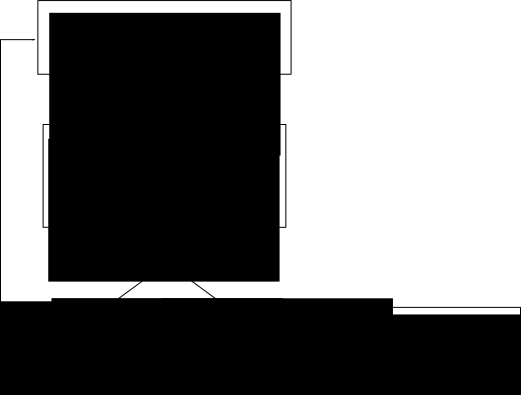
\includegraphics[width=0.6\textwidth]{\Curie/figs/diagrama-de-flujo.pdf}
\caption{Diagrama de Flujo del algoritmo desarrollado para el c�lculo de Profundidades de Curie.}
\label{fig-curie-diagrama-de-flujo}
\end{figure}

\subsection{Selecci�n de Ventana de Anomal�as}
Como datos de entrada tomamos valores de anomal�as magn�ticas situados en una grilla regular en coordenadas planas, es decir, las distancias entre los puntos deben estar en metros. El software desarrollado nos da acceso a una sencilla interfaz gr�fica que nos permite seleccionar una ventana cuadrada de puntos de anomal�a con la que deseamos trabajar. Su centro ser� el punto en el cual asociaremos luego la profundidad que obtengamos. Para no tener inconvenientes con la determinaci�n del mismo, el ancho de la ventana tendr� siempre un n�mero impar de puntos.

Adem�s de determinar la ubicaci�n de la ventana, la interfaz nos permite redimensionarla, aumentando o disminuyendo su ancho. Una vez seleccionada, procedemos a calcular el promedio radial del espectro de potencia. 

\subsection{C�lculo del Espectro de Potencias y Promedio Radial}
Al inicio el software nos pide especificar la cantidad de puntos que deseamos que nuestro espectro posea. Con la ventana ya seleccionada, el software autom�ticamente calcula cu�ntos puntos de padding cero que necesita agregar para que el espectro posea dicha cantidad de puntos; y luego modifica la ventana de anomal�as con el padding necesario.

La Transformada de Fourier de la nueva ventana se lleva a cabo a trav�s de la funci�n fftpack.fft2 de SciPy (\cite{SciPy}) y luego se calcula el espectro de potencia simplemente con el cuadrado del m�dulo de los valores. De este proceso se obtiene una grilla en el espacio de frecuencias $(k_x, k_y)$ con valores positivos o nulos. Cerca del origen de coordenadas se ubica la informaci�n de bajas frecuencias; mientras que a medida que nos movemos hacia los extremos, las mismas aumentan.

Para calcular el Promedio Radial dividimos la grilla de frecuencias en anillos conc�ntricos con centro en el origen. La cantidad de anillos ser� la mitad de los puntos por eje de la grilla. Luego promediamos los valores de anomal�as que caigan dentro de cada anillo. De esta forma obtenemos el promedio radial del espectro de potencia por cada anillo; y como cada uno posee una frecuencia media (radio medio en el espacio de frecuencias), se construye as� una gr�fica en 1 dimensi�n a partir de nuestro espectro de potencia. Adem�s de los valores del promedio radial, calculamos tambi�n la desviaci�n est�ndar en cada anillo, con lo cual obtenemos un intervalo de error por cada punto del promedio radial.

Luego, analizamos gr�ficamente el logaritmo de la curva obtenida verificando si se asemeja a simple vista a la propuesta de \cite{Blakely1995}, en otras palabras, si presenta un pico y luego un comportamiento lineal decreciente. De no ser as� debemos seleccionar otra ventana y proceder de la misma manera. Si por el contrario, la ventana aparenta ser ajustable, procedemos al siguiente paso.

\subsection{Ajuste de la Curva}
El ajuste del logaritmo del promedio radial del espectro de potencias se realiza sencillamente a trav�s del algoritmo de Levenberg-Marquardt, mediante su implementaci�n en la funci�n curve\_fit de SciPy. Habiendo seleccionado previamente los puntos con los cuales queremos que la curva ajuste, los cuales en general coinciden con los de bajas frecuencias.

Como salida de este m�todo obtenemos las profundidades $Z_{t}$ y $Z_{b}$ que mejor ajustan junto con la constante aditiva $\ln A$ y los errores de esos valores. Es importante analizar si el ajuste es satisfactorio, ya que puede suceder que la curva obtenida se correlacione con los puntos seleccionados, pero el error relativo de las profundidades sea muy elevado, dando un intervalo de confianza muy amplio como para considerar dicha estimaci�n como un buen resultado.

A�n as�, es com�n ver en la bibliograf�a que los errores en las Profundidades de Curie suelen ser elevados, incluso rondando entre el 10\% y el 20\%. Por ende, podemos esperar encontrarnos con cifras en ese orden.


\subsection{Interfaz Interactiva}
En la Figura \ref{fig-cudepy-muestra-1} se muestra la interfaz del software que permite la selecci�n de la ventana de anomal�as. En el gr�fico de la derecha podemos seleccionar interactivamente la ventana que deseamos y luego ordenarle que nos muestre, en los ejes de la izquierda, el promedio radial del espectro de las anomal�as interiores a dicha ventana.

Si deseamos tomar ese espectro para realizar el ajuste de la curva, continuamos al siguiente paso: elegir qu� puntos de la gr�fica utilizaremos como entrada. Un ejemplo de esto se muestra en la Figura \ref{fig-cudepy-muestra-2} a. Una vez ajustado, el software nos muestra los valores de los par�metros $Z_{t}$ y $Z_{b}$ y la curva de ajuste correspondiente, como se expone en la Figura \ref{fig-cudepy-muestra-2} b. Adem�s, nos da informaci�n de los errores de estos par�metros, y nos alerta en caso de que el error relativo de la Profundidad de Curie $Z_{b}$ sea mayor al 40\%.

%~ \newpage
\begin{figure}[h!]
\centering
\includegraphics[width=0.98\textwidth]{\Curie/figs/CuDePy-muestra-1.pdf}
\caption{Interfaz Interactiva para la selecci�n de ventana de anomal�as. A la derecha se ve la grilla de anomal�as magn�ticas junto con la regi�n seleccionada para conformar la ventana. A la izquierda se ve el logaritmo del promedio radial del espectro de potencias, habiendo aplicado el padding necesario para tener 70 puntos en dicha gr�fica. En este ejemplo se tom� una ventana de 30km de ancho.}
\label{fig-cudepy-muestra-1}
\end{figure}

\begin{figure}[h!]
\centering
\includegraphics[width=0.98\textwidth]{\Curie/figs/CuDePy-muestra-2.pdf}
\caption{(a) Ventana para seleccionar los puntos con los cuales deseamos hacer el ajuste de la curva, a partir del espectro obtenido en el ejemplo de la Figura \ref{fig-cudepy-muestra-1}. (b) Curva de ajuste de dichos puntos. En rojo se muestran aquellos que han sido elegidos para el ajuste. Los par�metros que se obtuvieron fueron: $Z_{t} = (3.6 \pm 0.6)$km y $Z_{b} = (5.9 \pm 1.3)$km.}
\label{fig-cudepy-muestra-2}
\end{figure}
\newpage{}

\section{Modelo sint�tico}
Con el objetivo de corroborar el funcionamiento del software desarollado, construimos un modelo sint�tico que consiste en una loza de 600km de ancho con profundidades $Z_{t}=5$km y $Z_{b}=25$km.


\begin{figure}[h!]
\centering
\includegraphics[width=0.99\textwidth]{\Curie/figs/sintetico-seleccion-ventana.png}
\caption{Interfaz gr�fica mostrando la selecci�n de la ventana de las anomal�as magn�ticas generada por el modelo sint�tico.}
\label{fig-curie-sintetico-seleccion-ventana}
\end{figure}

\begin{figure}[h!]
\centering
\includegraphics[width=0.75\textwidth]{\Curie/figs/sintetico-ajuste-curva.pdf}
\caption{Espectro de Potencia de la ventana seleccionada en la Figura \ref{fig-curie-sintetico-seleccion-ventana} junto con la curva de ajuste. Las profundidades obtenidas fueron de $Z_{t}= (5.0 \pm 0.2)$km y $Z_{b} = (25 \pm 2)$km.}
\label{fig-curie-sintetico-ajuste-curva}
\end{figure}

Para simular el comportamiento aleatorio de la magnetizaci�n $M(x,y)$
la loza est� constituida por 2020$\times$2020 prismas de aproximadamente 300m de ancho, que se extienden verticalmente desde $Z_{t}$ hasta $Z_{b}$ y cada uno cuenta con una magnetizaci�n aleatoria con distribuci�n uniforme entre -1 y 1 [A/m], verticalmente orientada.

Luego, a trav�s de funciones de la librer�a Fatiando a Terra (\cite{Uieda2014}), calculamos la anomal�a que esta loza genera en una grilla de 101$\times$101 nodos con un equiespaciado de 3km, ubicada en $z=0$, de tal forma que el origen de la grilla coincide con el origen (en $(x,y)$) de la loza. En la Figura \ref{fig-curie-sintetico-seleccion-ventana} se expone la interfaz de CuDePy, en la cual se puede observar la anomal�a generada por la loza y a su izquierda el espectro de la ventana seleccionada.

En la Figura \ref{fig-curie-sintetico-ajuste-curva} mostramos el espectro junto con la curva de ajuste. Los par�metros que se obtuvieron para este modelo sint�tico fueron: $Z_{t}= (5.0 \pm 0.2)$km y $Z_{b} = (25 \pm 2)$km. Demostrando as� que el software desarrollado reproduce con buena precisi�n al modelo sint�tico propuesto.

Vale observar que la profundidad de Curie que obtuvimos, en un caso muy ideal, posee un error relativo del orden del 10\%. Esto debe tomarse como una buena medici�n del par�metro $Z_{b}$. Como se mencion� en p�rrafos anteriores, es usual encontrarse con valores de error bastante elevados en la determinaci�n de las profundidades de la loza, especialmente en el $Z_{b}$.

\prechapterpage
\chapter{Aplicaci�n del M�todo}

\section{En La Payunia}
EL bloque San Rafael y Payunia se encuentran ubicados en el centro-sur de la Provincia de Mendoza (ver Figura \ref{fig-curie-payunia}). En ella podemos hallar dos volcanes importantes: el Pay�n Matr� y el Cerro Nevado, que presentan un magmatismo joven de composici�n primordialmente bas�ltica.

Tomando los datos de anomal�a magn�ticas obtenidos por \cite{Anci2012}, aplicamos el m�todo desarrollado para obtener la Profundidad del Punto de Curie en esta zona. Hemos sido capaces de ajustar satisfactoriamente dicho valor en 29 ventanas diferentes, con un error promedio del 20$\%$. El ancho de las ventanas utilizadas variaba seg�n la profundidad del Punto de Curie en cada una de ellas. Para regiones donde el $Z_{b}$ era m�s superficial utilizamos ventanas del orden de los 30km, mientras que para las que presentaban valores m�s profundos, el mismo rondaba los 60km.

\begin{figure}[b!]
    \centering{}
    \includegraphics[width=1\textwidth]{\Curie/figs/curie-payunia.pdf}
    \caption{Grillas de Anomal�a Magn�tica para la regi�n de Payunia junto a la grilla de Profundidades de Curie calculadas. Se pueden identificar el volc�n Pay�n Matr� (el m�s austral) y el Cerro Nevado.}
    \label{fig-curie-payunia}
\end{figure}

Como resultado obtuvimos la grilla de Profundiades del Punto de Curie que se muestra en la Figura \ref{fig-curie-payunia}, en la cual podemos diferenciar una regi�n m�s caliente hacia el este, y otra m�s fr�a hacia el oeste. Cuanto m�s superficial se encuentra el Punto de Curie entendemos que la regi�n es m�s c�lida, ya que la isoterma se encuentra m�s cerca de la superficie terrestre. Estos resultados est�n de acuerdo con la geolog�a de la zona: en la regi�n volc�nica la isoterma es m�s superficial debido al flujo t�rmico que las c�maras magm�ticas generan.


\section{En Vinchina}

\begin{figure}[b!]
    \centering
    \begin{subfigure}[h]{0.49\textwidth}
        \includegraphics[width=\textwidth]{\Curie/figs/ceci-anomalia.jpg}
    \end{subfigure}
    \begin{subfigure}[h]{0.49\textwidth}
        \includegraphics[width=\textwidth]{\Curie/figs/ceci-curie.jpg}
    \end{subfigure}
    \caption{Grillas de Anomal�a Magn�tica para la regi�n de Vinchina junto a la grilla de Profundidades de Curie calculadas por \cite{Weidmann2015}.}
    \label{fig-curie-vinchina}
\end{figure}

El m�todo aqu� desarrollado fue puesto a disposici�n de \cite{Weidmann2015} con el fin de aplicarlo en la zona de estudio que involucra su trabajo de Tesis. La misma consiste en la Cuenca de Vinchina, ubicada en la Regi�n de los Andes Centrales, sobre la zona de subducci�n subhorizontal de la placa oce�nica de Nazca (ver Figura \ref{fig-curie-vinchina}).




En esta regi�n, se han interpretado importantes colisiones de terrenos, que han causado grandes orog�nesis dentro del Gondwana. Los modelos geol�gicos-geof�sicos  indican la existencia de una importante estructura geol�gica de alta densidad, ubicada bajo la cuenca de Vinchina,  que se podr�a vincular con un sector del arco Famatiniano y la cu�a de acreci�n de Cuyania y Gondwana. Resultando ser una cuenca fr�a y inmadura.

Los resultados obtenidos mediante la aplicaci�n del software aqu� desarrollado se pueden ver en la Figura \ref{fig-curie-vinchina}, los cuales refuerzan las interpretaciones mencionadas en el p�rrafo anterior.



\prepartpage
\part[Determinaci�n del Espesor El�stico]{Determinaci�n del Espesor El�stico de la Corteza Terrestre}

\chapter{Isostasia Flexural}

%~ \vspace{1cm}

Los modelos isost�ticos cl�sicos, como el de Airy o el de Pratt, pueden clasificarse dentro de los llamados modelos locales. Esto se debe a que una columna topogr�fica de altura $h$ solo afecta a la columna subyacente generando una ra�z que se deflecta una profundidad $w$. La presencia de esa columna no modifica en absoluto la profundidad de la ra�z en regiones vecinas.

Esto fue discutido por Vening Meinesz, quien cre�a que la compensaci�n de la superficie terrestre no necesariamente deb�a ser local. En cambio, propuso un modelo de isostasia regional, en el cual la corteza terrestre se comporta como una placa el�stica (en escala de tiempos geol�gicos) que flota sobre un sustrato no viscoso y la topograf�a puede considerarse como una carga que genera la deflexi�n de la placa, explicando as� la presencia de la ra�z.

Esta placa el�stica tendr� una propiedad que se conoce como rigidez flexural, la cual define qu� tan r�gida es la placa. Cu�nto mayor es este valor, la isostasia ser� m�s regional. M�s adelante mostraremos que esta magnitud depende de par�metros como los m�dulos de Young y de Poisson de la placa y a su vez de su espesor.

Al aplicar el modelo a la lit�sfera, definimos el Espesor El�stico de la corteza como el espesor que deber�a tener una placa el�stica de m�dulo de Young $E=1\cdot 10^{11}\,{\rm Pa}$ y m�dulo de Poisson $\nu = 0.25$ para generar la misma deflexi�n que presenta la corteza.

Vale observar que el espesor el�stico resulta una propiedad virtual de la corteza, o bien, un par�metro de un modelo an�logo a ella. Sin embargo, el an�lisis de las variaciones del espesor el�stico permite identificar elementos de la reolog�a de la misma, as� como hallar estructuras internas o variaciones t�rmicas, hasta obtener informaci�n sobre la edad de las placas.

Actualmente existen diversos m�todos para la determinaci�n del espesor el�stico, siendo todos muy discutidos. Aqu� presentaremos un m�todo espectral que recopila aspectos de varios de los m�todos ya existentes con el objetivo de mejorar el an�lisis de los resultados y disminuir los tiempos de c�mputo.

A continuaci�n describiremos el modelo de placa delgada, a trav�s del cual interpretamos el espesor el�stico de la corteza.

\vspace{2cm}

\section{Modelo El�stico de Placa Delgada}
\label{section-modelo-placa-delgada}
Consideremos una placa de espesor $T_{e}$, largo $L$ y extendida infinitamente en el eje $z$ que se encuentra fija en sus extremos y bajo la acci�n de una fuerza por unidad de area $q(x)$ aplicada a lo largo de largo de la misma (ver Figura \ref{fig-placa-delgada-1}).

Vamos a suponer que la placa es delgada, es decir, que su largo es mucho mayor que su espesor ($L \gg T_{e}$) y que posee un comportamiento el�stico, el cual podemos garantizar exigiendo que la deflexi�n $w$ que presenta la placa, debido a la presencia de la fuerza $q(x)$, sea mucho m�s peque�a que su largo ($L \gg w$).

\begin{figure}[b!]
\centering
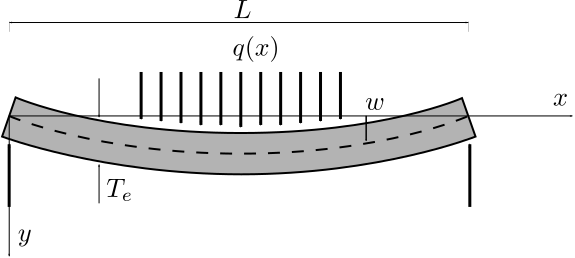
\includegraphics[width=0.9\textwidth]{\Flexion/figs/placa-delgada-1.pdf}
\caption{Esquema de la placa delgada propuesta.}
\label{fig-placa-delgada-1}
\end{figure}

Bajo estas hip�tesis, analicemos el balance de fuerzas y momentos sobre una porci�n infinitesimal de la placa de longitud $dx$. En �l actuar� una fuerza $q(x)\,dx$ sobre la superficie superior debido a la carga $q(x)$ y unas fuerzas netas de corte (shear) por unidad de longitud $V$ y $V + dV$ en sus caras verticales, respectivamente. Adem�s, debido a las tensiones normales (normal stress $\sigma_{xx}$) aparecen momentos resultantes por unidad de longitud $M$ y $M + dM$ en las caras verticales, respectivamente. Estas fuerzas y momentos est�n esquematizadas en la Figura \ref{fig-placa-delgada-2}. Como es de esperarse, la deflexi�n $w$ var�a a lo largo de la placa, por lo cual en cada cara vertical de la porci�n infinitesimal tendremos dos deflexiones: $w$ y $w+dw$, respectivamente.

Realizando el balance de fuerzas en el eje $y$ obtenemos que:
\begin{equation}
    q(x)\, dx + (V + dV) - V = 0 \quad \Rightarrow \quad q(x)\,dx + dV = 0 \\
\end{equation}
\begin{equation}
    \therefore \,\, q(x) = -\frac{dV}{dx}
    \label{eq-placa-delgada-q-V}
\end{equation}

Realizando el balance de momentos obtenemos:
\begin{equation}
    M - (M+dM) + \frac{1}{2} V dx + \frac{1}{2}(V+dV)dx = 0
\end{equation}
\begin{equation}
    \therefore \,\, \frac{dM}{dx} = V
    \label{eq-placa-delgada-M-V}
\end{equation}


\begin{figure}[t!]
\centering
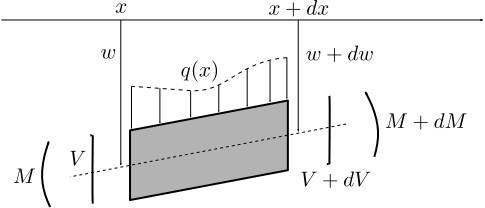
\includegraphics[width=0.75\textwidth]{\Flexion/figs/placa-delgada-2.pdf}
\caption{Porci�n infinitesimal de la placa delgada.}
\label{fig-placa-delgada-2}
\end{figure}

Derivando la ecuaci�n anterior y utilizando la relaci�n \ref{eq-placa-delgada-q-V}, podemos arribar a la siguiente relaci�n entre el momento $M$ y la carga $q(x)$:
\begin{equation}
    \therefore \,\, \frac{d^2 M}{dx^2} = -q(x)
    \label{eq-momento-carga}
\end{equation}

Veamos c�mo podemos relacionar al momento $M$ con la deflexi�n $w$ para as� transformar la ecuaci�n anterior en una ecuaci�n diferencial que relacione la carga $q(x)$ con la deflexi�n de la placa.

El momento $M$ lo podemos calcular como la sumatoria de los momentos generados por todas las tensiones normales aplicadas en una cara vertical:
\begin{equation}
    M = \int\limits_{-T_{e}/2}^{T_{e}/2} \!\! \sigma_{xx} \, y' dy'
\end{equation}

\begin{figure}[b!]
\centering
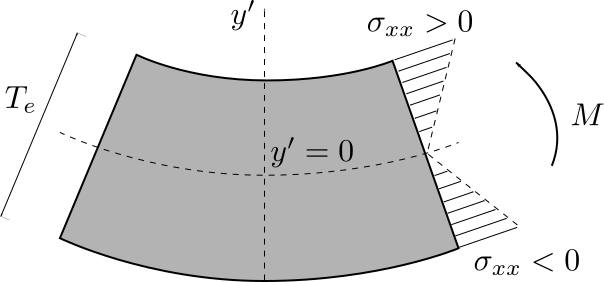
\includegraphics[width=0.6\textwidth]{\Flexion/figs/placa-delgada-3.pdf}
\caption{Esquema de las tensiones normales (normal stress) en un corte de la placa.}
\label{fig-placa-delgada-3}
\end{figure}



Si la placa se deflecta hacia abajo, la cara superior se contrae y la tensi�n normal es positiva desde el centro de la placa hacia arriba, mientras que la cara inferior se dilata y la tensi�n normal desde el centro hacia abajo es negativa, como se puede ver en la Figura \ref{fig-placa-delgada-3}.

La relaci�n entre la tensi�n normal $\sigma_{xx}$ y la dilataci�n o contracci�n de la placa viene dada por la Ley de Hooke. Considerando que las tensiones normales $\sigma_{xx}$ generan una deformaci�n $\varepsilon_{xx}$ en la misma direcci�n; que no existen deformaciones en direcciones perpendiculares al plano $xy$ ya que en $z$ la placa se extiende infinitamente; y que podemos despreciar las tensiones $\sigma_{yy}$ debido a la aproximaci�n de placa delgada, podemos escribir entonces la tensi�n $\sigma_{xx}$ en funci�n de la deformaci�n $\varepsilon_{xx}$:
\begin{equation}
    \sigma_{xx} = \frac{E}{1-\nu^{2}} \, \varepsilon_{xx}
\end{equation}
donde $E$ y $\nu$ son el m�dulo de Young y el de Poisson de la placa, respectivamente.

Tras un an�lisis geom�trico \cite[p. 203-204]{Turcotte2001} es posible relacionar la deformaci�n $\varepsilon_{xx}$ con la deflexi�n de la placa:
\begin{equation}
    \varepsilon_{xx} (y') = -y' \, \frac{d^{2} w}{dx^{2}}
\end{equation}

Agrupando la informaci�n de las �ltimas tres ecuaciones podemos reescribir al momento $M$ como:
\begin{equation}
    M = - \frac{E}{1-\nu^{2}} \, \frac{d^{2} w}{dx^{2}} \int\limits_{-T_{e}/2}^{T_{e}/2} \!\! {y'}^{2} dy' = - \frac{E \, T_{e}^{\,3}}{12 (1-\nu^{2})} \, \frac{d^{2} w}{dx^{2}}
\end{equation}

Definimos la rigidez flexural $D$ como:
\begin{equation}
    \boxed{ D \equiv \frac{E \, T_{e}^{\,3}}{12 (1-\nu^{2})} } 
    \label{eq-rigidez-flexural}
\end{equation}
entonces, la relaci�n entre el momento $M$ y la flexi�n de la placa $w$ queda determinada por la siguiente ecuaci�n diferencial:
\begin{equation}
    M = -D \, \frac{d^{2}w}{dx^{2}}
\end{equation}

Remplazando finalmente la �ltima expresi�n del momento $M$ en la ecuaci�n \ref{eq-momento-carga} obtenemos la ecuaci�n diferencial que relaciona la carga $q(x)$ con la deflexi�n $w(x)$ que esta genera:
\begin{equation}
    \frac{d^{2}}{dx^{2}} \left[ D \, \frac{d^{2} w}{dx^{2}} \right] = q(x)
\end{equation}

Y si adem�s suponemos que la rigidez flexural es constante a lo largo de toda la placa, entonces la ecuaci�n anterior puede escribirse como:
\begin{equation}
    \therefore \,\, \boxed{D \, \frac{d^{4}w}{dx^{4}} = q(x)}
    \label{eq-deflexion-carga}
\end{equation}

\newpage{}
\section{Aplicaci�n al Modelado de la Lit�sfera}
A la hora de modelizar la corteza como si se tratase de una placa el�stica y delgada, es necesario tener en cuenta ciertas cuestiones. Nuestro modelo partir� de una lit�sfera normal, es decir, una corteza de ancho $t$ que flota sobre un manto no viscoso (ver Figura \ref{fig-litosfera-fuerza-q}a). Al incorporar topograf�a a este esquema, estas ser�n consideradas como cargas, tal y como lo hac�amos con las fuerzas por unidad de superficie $q(x)$. Esta topograf�a producir� una deflexi�n en la corteza, generando as� la aparici�n de la ra�z.

\begin{figure}[b!]
    \centering{}
    \includegraphics[width=0.98\textwidth]{\Flexion/figs/litosfera-fuerza-q.pdf}
    \caption{$(a)$ Esquema del modelo de partida para desarrollar la isostasia flexural en lit�sfera. $(b)$ Al incorporar una carga topogr�fica al escenario anterior, aparece una ra�z que se deflecta hacia abajo para compensar dicha carga. $(c)$ Comprimimos toda la carga topogr�fica en una fuerza $q_{a}$ por unidad de �rea. $(d)$ Columna de la lit�sfera para evaluar la fuerza total $q$ como sumatoria de las cargas topogr�ficas y las enterradas.}
    \label{fig-litosfera-fuerza-q}
\end{figure}

Sin embargo, cuando esta �ltima desplaza parte del manto, genera una fuerza hidrost�tica que intentar� restaurarla a su posici�n original. Es por ello que dentro de la carga $q(x)$ deberemos incorporar tanto las cargas topogr�ficas como las fuerzas hidrost�ticas (conocidas tambi�n como cargas enterradas).

Llamemos $q_{a}$ a la fuerza por unidad de �rea generada �nicamente por la carga topogr�fica y consideremos una columna de la lit�sfera (ver Figura \ref{fig-litosfera-fuerza-q}c). Calculemos la carga total $q$ como sumatoria de las cargas topogr�ficas y las enterradas. Por un lado tenemos el peso por unidad de �rea de cada uno de los elementos de la columna:
\begin{equation}
    \rho_{c}(t+w)g + \rho_{m}h_{m}\,g
\end{equation}

Y por otro la presi�n  en la base de la columna:
\begin{equation}
    \rho_{c}\, tg + \rho_{m}(w+h_{m})g
\end{equation}

A�adiendo la carga topogr�fica $q_{a}$, la fuerza total $q$ queda determinada:
\begin{gather}
    q = q_{a} + \Big[ \rho_{c}(t+w)g + \rho_{m}h_{m}\, g \Big] - \Big[ \rho_{c}\, tg + \rho_{m}(w+h_{m})g \Big] \\[2ex]
    \therefore \,\, q(x) =  q_{a}(x) - \underbrace{(\rho_{m}-\rho_{c})g\, w(x) }_{\mathclap{\textrm{fuerza hidrost�tica restauradora}}}
\end{gather}


Reemplazando esta expresi�n de $q(x)$ en la ecuaci�n \ref{eq-deflexion-carga} obtenemos:
\begin{equation}
    \therefore \,\, D \, \frac{d^{4}w}{dx^{4}} + (\rho_{m} - \rho_{c})g\, w(x) = q_{a}(x)
\end{equation}

Finalmente, si consideramos que la topograf�a posee una densidad constante de $\rho_{t}$, entonces podemos reemplazar a $q_{a}$ por:
\begin{equation}
    q_{a}(x) = \rho_{t}g \, h(x)
\end{equation}
donde $h(x)$ es la cota topogr�fica en el punto $x$. Y por ende la ecuaci�n diferencial queda expresada como:

\begin{equation}
    \therefore \,\, \boxed{ D \, \frac{d^{4}w}{dx^{4}} + (\rho_{m} - \rho_{c})g\, w(x) = \rho_{t}g\, h(x) }
    \label{eq-deflexion-litosfera}
\end{equation}

Esta ecuaci�n diferencial nos permite obtener la deflexi�n de la ra�z $w(x)$ de una corteza con rigidez flexural $D$ generada por una carga topogr�fica $q_{a}(x)$. La �nica dificultad que tendr�amos ser�a la capacidad de resoluci�n de dicha ecuaci�n. Una opci�n puede ser encararla a trav�s de diferencias finitas, sin embargo, veremos m�s adelante que es posible trasladar el problema al espacio de frecuencias, donde adem�s tendremos una mejor interpretaci�n del comportamiento del sistema.

\section{Isostasia Flexural como Filtro de Frecuencias}
Con el fin de interpretar el comportamiento de la ra�z frente a cargas topogr�ficas y de obtener un m�todo de resoluci�n r�pida de la ecuaci�n diferencial \ref{eq-deflexion-litosfera}, trasladaremos el problema al espacio de frecuencias. Para ello aplicamos la Transformada de Fourier en cada miembro de la ecuaci�n antes nombrada.

\begin{multline}
    \mathcal{F} \Bigg[ D \, \frac{d^{4}w}{dx^{4}} + (\rho_{m} - \rho_{c})g\, w(x) \Bigg] = \mathcal{F} \Big[ \rho_{t}g\, h(x) \Big] \quad \Rightarrow \\
    D \, \mathcal{F} \Big[ \frac{d^{4}w}{dx^{4}} \Big] + (\rho_{m} - \rho_{c})g\,\mathcal{F} \Big[ w(x) \Big] = \rho_{t}g \, \mathcal{F} \Big[ h(x) \Big]
\end{multline}


Vamos a llamar $W(k)$ y $H(k)$ a las Transformadas de Fourier de la deflexi�n $w(x)$ y la topograf�a $h(x)$, respectivamente. Adem�s, haciendo uso de la propiedad de la ecuaci�n \ref{eq-transformada-de-la-derivada}, la ecuaci�n diferencial queda reescrita en el espacio de frecuencias como:

\begin{multline}
    \left[ Dk^{4} + (\rho_{m} - \rho_{c})g \right]\, W(k) = \rho_{t}g \, H(k) \quad \Rightarrow \\
    W(k) = \frac{\rho_{t}g}{Dk^{4} + (\rho_{m}-\rho_{c})g}\, H(k)
\label{eq-deflexion-frecuencias-1}
\end{multline}

Definiendo la funci�n $\Phi_{e}(k)$ como:
\begin{equation}
    \Phi_{e}(k) \equiv \Bigg[ \frac{Dk^{4}}{(\rho_{m}-\rho_{c})g} +1 \Bigg]^{-1}
    \label{eq-filtro-phi}
\end{equation}

Podemos reescribir la ecuaci�n \ref{eq-deflexion-frecuencias-1} de la siguiente manera:
\begin{equation}
    \therefore \,\, \boxed{ W(k) = \frac{\rho_{t}}{\rho_{m}-\rho_{c}} \, \Phi_{e}(k) \, H(k) }
    \label{eq-deflexion-topografia-freq-1d}
\end{equation}

De esta forma, conociendo las densidades involucradas y la rigidez flexural de la placa, es posible obtener la Transformada de Fourier de la deflexi�n de la corteza s�lo a partir de la cota topogr�fica. La obtenci�n de la deflexi�n $w(x)$ se reduce �nicamente a antitransformar la $W(k)$ obtenida.

La ecuaci�n anterior no solo nos brinda una sencilla forma de resoluci�n de la isostasia flexural, sino que adem�s nos permite interpretar la obtenci�n de la deflexi�n como un filtrado de frecuencias de la topograf�a, realizado a trav�s de la funci�n $\Phi_{e}(k)$.

En la Figura \ref{fig-filtro-phi} se observa una gr�fica de $\Phi_{e}(k)$ para distintos valores de rigidez flexural. En ella se puede apreciar que el filtro se comporta como un pasabajos, atenuando el efecto de las altas frecuencias y manteniendo el de las m�s bajas. Adem�s, podemos ver que cu�nto mayor es la rigidez $D$, m�s estricto es el filtro.


\begin{figure}[b!]
    \centering{}
    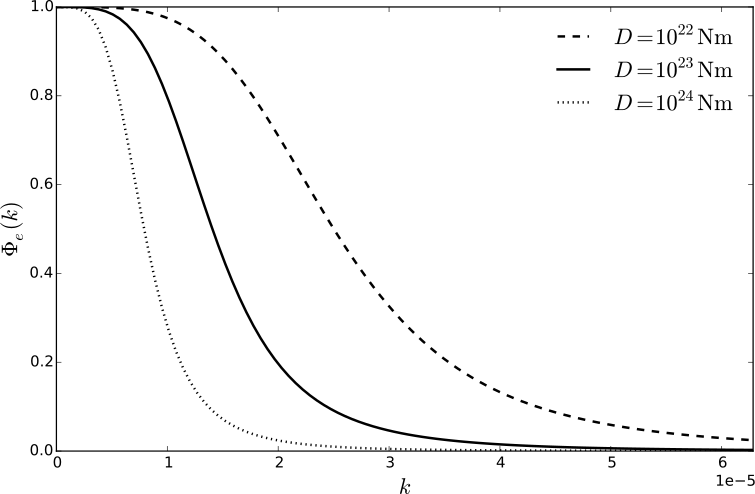
\includegraphics[width=0.7\textwidth]{\Flexion/figs/filtro_phi.pdf}
    \caption{Gr�fica del filtro $\Phi_{e}(k)$ para distintos valores de rigidez flexural. Se puede corroborar que efectivamente se comporta como un pasabajos y que cu�nto mayor es el valor de $D$, m�s estricto es el filtro.}
    \label{fig-filtro-phi}
\end{figure}


En la Figura \ref{fig-deflexiones} podemos ver una topograf�a arbitraria con densidad $\rho_{t} = 2670$kg/m$^{3}$ en una corteza de densidad $\rho_{c} = 2900$kg/m$^{3}$ y ancho $t=35$km. Y por debajo de ella se muestran las distintas ra�ces que se obtienen para diferentes valores de espesor el�stico $T_{e}$.

En el caso particular en el que la placa no tiene rigidez ($D=0$), el filtro $\Phi_{e}(k)$ es igual a la identidad y por ende se recupera el modelo isost�tico de Airy (ecuaci�n \ref{eq-airy}). Observando la gr�fica de la Figura \ref{fig-deflexiones} podemos ver que el Moho generado con $T_{e}=0$ coincide con el modelo isost�tico de Airy, generando una ra�z local. Mientras que los modelos flexurales producen que las ra�ces sean regionales y no reproduzcan el efecto de las altas frecuencias, como es el caso del pico que podemos ver en la topograf�a propuesta en dicha Figura.

\begin{figure}[t!]
    \centering{}
    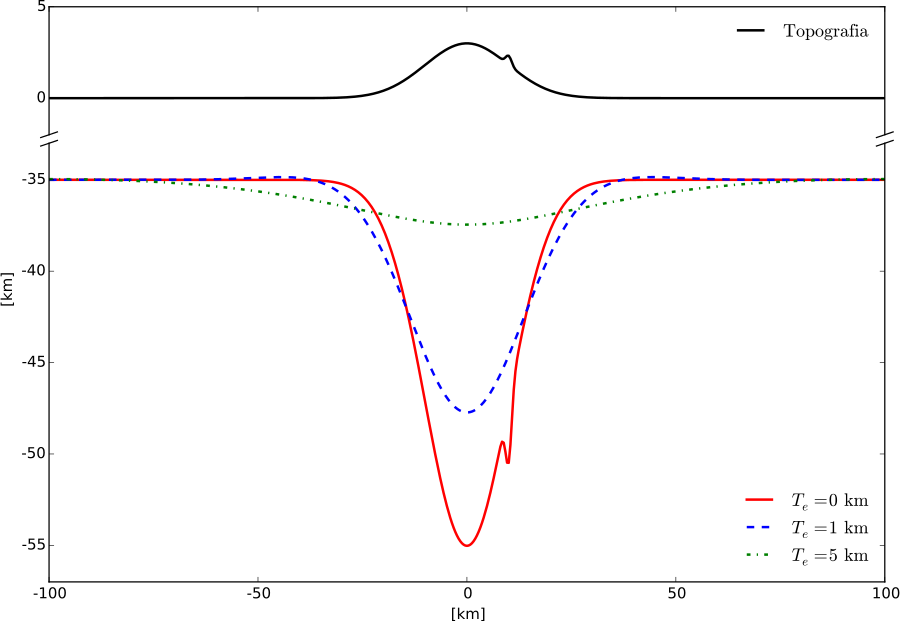
\includegraphics[width=0.98\textwidth]{\Flexion/figs/deflexiones.pdf}
    \caption{Perfil de lit�sfera con topograf�a arbitraria de densidad 2670kg/m$^{3}$, sostenida por una corteza normal de 35km de ancho y densidad 2900kg/m$^{3}$ sobre un manto de 3300kg/m$^{3}$. Se muestran los Mohos que se obtienen al aplicar un modelo de isostasia flexural para distintos valores de espesor el�stico $T_{e}$. El $T_{e}=0$ coincide con el modelo isost�tico de Airy.}
    \label{fig-deflexiones}
\end{figure}


\section{Generalizaci�n del Modelo}
El modelo propuesto en la secci�n \ref{section-modelo-placa-delgada} supone que las cargas est�n homogeneamente distribuidas a lo largo del eje $z$, pudiendo reducir el estudio de la deflexi�n de la corteza a una funci�n unidimiensional $w(x)$. Sin embargo, en la pr�ctica, las masas se encuentran distribuidas en todo el plano $xy$ heterogeneamente, por ende la deflexi�n vendr� dada por una funci�n $w(x, y)$ como soluci�n de una ecuaci�n diferencial a derivadas parciales.

Adem�s, la rigidez de la corteza no suele ser constante para regiones amplias, sino que pueden presentar variaciones, por lo tanto, es posible representarla mediante una funci�n $D(x, y)$.

La ecuaci�n diferencial que determina la ra�z para cargas distribuidas en el plano $xy$ y rigidez flexural variable es la siguiente (\cite{Garcia2014}):
\begin{equation}
    \nabla^{2} \left[ D\, \nabla^{2} w \right] - (1-\nu) \left[ \frac{\partial^{2} D}{\partial x^{2}} \, \frac{\partial^{2} w}{\partial y^{2}} - 2 \frac{\partial^{2} D}{\partial x \partial y} \, \frac{\partial^{2} w}{\partial x \partial y} + \frac{\partial^{2} D}{\partial y^{2}} \, \frac{\partial^{2} w}{\partial x^{2}} \right] + (\rho_{m}-\rho_{c})g\, w = \rho_{t}g \, h
    \label{eq-garcia}
\end{equation}

En el caso particular de que $D$ sea constante en toda la regi�n, la ecuaci�n diferencial se reduce a:
\begin{equation}
    D \, \nabla^{4} w + (\rho_{m}-\rho_{c})g\, w = \rho_{t}g \, h
\end{equation}

Y aplicando la Transformada de Fourier en esta ecuaci�n, se obtiene una relaci�n similar a la de \ref{eq-deflexion-topografia-freq-1d}:
\begin{equation}
    \boxed {W(k_{x}, k_{y}) = \frac{\rho_{t}}{\rho_{m}-\rho_{c}} \, \Phi_{e}(k) \, H(k_{x}, k_{y}) }
    \label{eq-deflexion-topografia-freq}
\end{equation}
donde $k$ es el m�dulo del vector ${\bf k} = (k_{x}, k_{y})$ y $\Phi_{e}(k)$ sigue estando definida seg�n la ecuaci�n \ref{eq-filtro-phi}.

\prechapterpage
\chapter{Inversi�n del Moho}

Nuestro objetivo es construir un m�todo que nos permita determinar el espesor el�stico de una regi�n de inter�s particular. De contar con datos de altura topogr�fica ($h$) y de profundidad del Moho en dicha zona ($t+w$), solo resta obtener el valor de $T_{e}$ que mejor ajusta la ecuaci�n \ref{eq-deflexion-topografia-freq}. Los datos de topograf�a son sencillos de recolectar a partir de modelos globales o mapas de elevaci�n digital; mientras que la profundidad del Moho se obtiene generalmente por sismolog�a. Sin embargo suele suceder que no tengamos mediciones sismol�gicas en nuestra zona de estudio.

En situaciones como esta es necesario hallar otra forma de calcular la profundidad del Moho. La opci�n que vamos a abordar aqu� reside en realizar una inversi�n de las anomal�as de Bouguer mediante m�todos espectrales.

En un trabajo que abri� nuevas puertas dentro de los m�todos espectrales en geof�sica, \cite{Parker1973} consider� el potencial gravitatorio producido por una capa de material de densidad $\rho$, cuyos l�mites inferior y superior son el plano $z=0$ y una superficie definida por $z = h({\bf r})$, respectivamente (con ${\bf r} = (x, y)$). Supuso que fuera de una regi�n finita, la placa se desvanece ($h({\bf r}) = 0 \,\, \forall \,\, r > R$, por ejemplo); y que $h$ es acotada e integrable. A partir de estas hip�tesis, obtuvo una expresi�n para la Transformada de Fourier de dicho potencial gravitatorio (medido en el plano de observaci�n $z = z_{0}$) como serie de potencias de la TF de $h({\bf r})$, modulada por una exponencial decreciente:
\begin{equation}
    \mathcal{F} \big[ U \big] = 2\pi G \rho \, e^{-kz_{0}} \, \sum\limits_{n=1}^{\infty} \frac{k^{\,n-2}}{n!} \mathcal{F} \big[ h^{n}({\bf r}) \big]
\end{equation}

Junto con una expresi�n an�loga para la componente en $z$ de la aceleraci�n de la gravedad, en el mismo plano de observaci�n:
\begin{equation}
    \mathcal{F} \big[\, g_{z} \,\big] = 2\pi G \rho \, e^{-kz_{0}} \, \sum\limits_{n=1}^{\infty} \frac{k^{\,n-1}}{n!} \mathcal{F} \big[ h^{n}({\bf r}) \big]
    \label{eq-parker-simple}
\end{equation}

Con estas ecuaciones elabor� tambi�n una soluci�n espectral para el problema de la continuaci�n ascendente, es decir, obtener la anomal�a gravitatoria $\Delta g'$ a un nivel $z'_{0}$ conociendo la anomal�a $\Delta g$ en un nivel $z_{0}$. Ya que si consideramos que ambas est�n generadas por los mismos cuerpos, responder�n a relaciones como la anterior a diferencia del factor del exponente ($z'_{0}$ y $z_{0}$ en cada caso). Es sencillo de calcular la relaci�n que existir� entre las TF de ambas anomal�as:
\begin{equation}
    \mathcal{F} \big[ \Delta g' \big] = e^{-(z'_{0}-z_{0})\, k} \, \mathcal{F} \big[ \Delta g \big]
\end{equation}

De esta forma obtuvo una soluci�n espectral muy simple, que se reduce a la aplicaci�n de un filtro pasabajos, a un problema que espacialmente debe encararse como la resoluci�n de una integral de superficie.

Finalmente, generaliz� la ecuaci�n \ref{eq-parker-simple} para una capa con l�mite superior $h({\bf r})$ e inferior $g({\bf r})$; y con densidad variable $\rho({\bf r})$:
\begin{equation}
    \mathcal{F} \big[\, g_{z} \,\big] = 2\pi G \, e^{-kz_{0}} \, \sum\limits_{n=1}^{\infty} \frac{k^{\,n-1}}{n!} \mathcal{F} \Big[ \rho({\bf r}) \big\{ h^{n}({\bf r}) - g^{n}({\bf r}) \big\} \Big]
    \label{eq-parker}
\end{equation}

\section{Modelo de Ra�z e Inversi�n de Anomal�as de Bouguer}
Para la inversi�n del Moho que propondremos vamos a considerar una ra�z de densidad constante con superficies superior e inferior $h({\bf r}) = -t$ y $g({\bf r}) = -[t + w({\bf r})]$ medidas desde $o$. La atracci�n gravitatoria que la ra�z genera se aproximar� mucho a la anomal�a de Bouguer, salvo por los cuerpos an�malos que puedan aparecer en corteza (ver Figura \ref{fig-anomalias-3-4}), asign�ndole una densidad equivalente al contraste entre las densidades del manto y la corteza. Tomaremos como hip�tesis para nuestro modelo que la �nica fuente de anomal�a de Bouguer es la ra�z propuesta con densidad constante $\rho_{c}-\rho_{m} < 0$.

Para simplificar los c�lculos, nos trasladamos al marco de referencia $o'$, en el cual las superficies de la ra�z vienen dadas por $h({\bf r'}) = 0$ y $g({\bf r'}) = - w({\bf r})$; y tomamos como plano de observaci�n de la anomal�a el $z=0$ ($z'=t$).

\begin{figure}[b!]
    \centering{}
    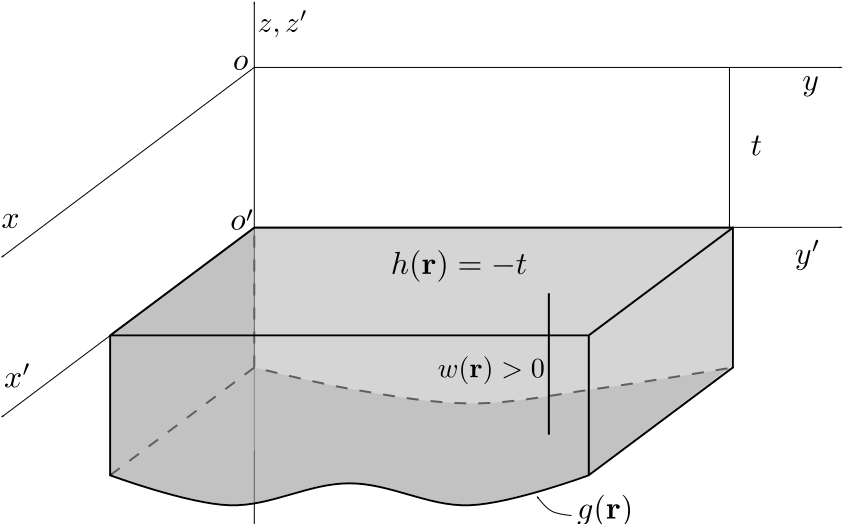
\includegraphics[width=0.7\textwidth]{\Flexion/figs/esquema-raiz.pdf}
    \caption{Modelo de ra�z con densidad constante para realizar la inversi�n del Moho a partir de anomal�as de Bouguer. Las superficies $h({\bf r})$ y $g({\bf r})$ medidas desde $o$ delimitan la ra�z superior e inferiormente, respectivamente. El ancho de la corteza normal es $t$ y $w({\bf r}) > 0$ es la deflexi�n de la misma.}
    \label{fig-esquema-raiz}
\end{figure}

Seg�n la ecuaci�n \ref{eq-parker}, la anomal�a de Bouguer estar� relacionada con las superficies que limitan la ra�z de la siguiente forma:
\begin{equation}
    \mathcal{F} \big[ \Delta g_{bg} \big] = -2\pi G \, (\rho_{m} - \rho_{c}) \,\, e^{-kt} \, \sum\limits_{n=1}^{\infty} \frac{k^{\,n-1}}{n!} \, \mathcal{F} \big[ \underbrace{ h^{n}({\bf r'}) }_{\mathclap{0^{n}}}  - \underbrace{ g^{n}({\bf r'}) }_{\mathclap{[-w({\bf r})]^{n}}} \big] \quad \Rightarrow
\end{equation}

\begin{equation}
    \mathcal{F} \big[ \Delta g_{bg} \big] = 2\pi G \, (\rho_{m} - \rho_{c}) \,\, e^{-kt} \, \sum\limits_{n=1}^{\infty} \frac{(-1)^{n}\,k^{\,n-1}}{n!} \, \mathcal{F} \big[ w^{n}({\bf r}) \big]
\end{equation}

Para llevar a cabo la inversi�n deseada tendremos que reordenar la ecuaci�n anterior, de forma an�loga a la propuesta por \cite{Oldenburg1974}; despejando el primer t�rmino de la sumatoria:
\begin{equation}
    \mathcal{F} \big[ w({\bf r}) \big] \,=\, - \frac{\mathcal{F} \big[ \Delta g_{bg} \big] \, e^{kt} }{2\pi G (\rho_{m}-\rho_{c})} \,\, +  \,\, \sum\limits_{n=2}^{\infty} \frac{(-1)^{n}\,k^{\,n-1}}{n!} \, \mathcal{F} \big[ w^{n}({\bf r}) \big]
    \label{eq-parker-oldenburg}
\end{equation}

Y luego construir un algoritmo iterativo que se retroalimente con la salida de la �ltima iteraci�n. Este m�todo fue desarrollado por \cite{Oldenburg1974} y se conoce como el m�todo de inversi�n de Parker-Oldenburg. Consiste en partir de una deflexi�n arbitraria $w_{0}$ y calcular la ra�z de la iteraci�n $i$ a partir de la obtenida en la iteraci�n $i-1$:
\begin{equation}
    \boxed{\mathcal{F} \big[\, w_{i} \,\big]  \,=\, \underbrace{ - \frac{\mathcal{F} \big[ \Delta g_{bg} \big] \, e^{kt} }{2\pi G (\rho_{m}-\rho_{c})}}_{\mathclap{\textrm{t�rmino constante}}} \,\, +  \,\, \sum\limits_{n=2}^{N} \frac{(-1)^{n}\,k^{\,n-1}}{n!} \, \mathcal{F} \big[\, w^{n}_{i-1} \,\big]}
    \label{eq-parker-oldenburg-iterativo}
\end{equation}
donde $N$ es el orden m�ximo de la sumatoria. Las iteraciones se llevan a cabo hasta que el sistema alcance un criterio de interrupci�n deseado. Notemos que el primer t�rmino de la ecuaci�n anterior no se ve modificado en ninguna de las iteraciones, es por ello que lo denominaremos t�rmino constante.

\begin{figure}[t!]
    \centering{}
    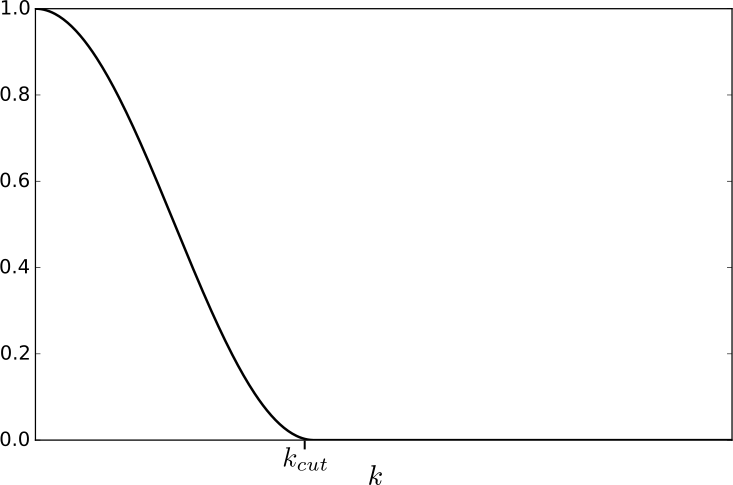
\includegraphics[width=0.65\textwidth]{\Flexion/figs/hamming-filter.pdf}
    \caption{Gr�fica del filtro pasabajos de Hamming, definido en la ecuaci�n \ref{eq-hamming-filter} y utilizado para eliminar las altas frecuencias en cada iteraci�n de la inversi�n del Moho mediante el m�todo Parker-Oldenburg.}
    \label{fig-hamming-filter}
\end{figure}

Un aspecto importante para asegurar la convergencia de este algoritmo es aplicar un filtro pasabajos entre cada iteraci�n (\cite{Oldenburg1974}, \cite{Braitenberg1999}, \cite{Braitenberg2000}, \cite{Gomez-Ortiz2005}). Esto se debe a que la exponencial creciente del t�rmino constante amplifica las altas frecuencias, lo cual dificulta la convergencia del algoritmo. Nuestra propuesta es utilizar un filtro que se conoce como filtro de Hamming:
\begin{equation}
    \textrm{Hamming}\,(k) = \left\{
    \begin{array}{cr}
        \frac{1}{2} \left[ 1 + \cos \left( \pi \frac{k}{k_{cut}} \right) \right] \quad & k<k_{cut}\\[2ex]
        0 \quad & k \ge k_{cut}
    \end{array}
    \right.{}
    \label{eq-hamming-filter}
\end{equation}

En la Figura \ref{eq-hamming-filter} se muestra una gr�fica de este filtro de frecuencias, donde se ve que $k_{cut}$ cumple la funci�n de una frecuencia de corte: se eliminan las contribuciones de frecuencias mayores a ella.



\section[Implementaci�n en Python del Algoritmo Parker-Oldenburg]{Implementaci�n en Python del Algoritmo\\Parker-Oldenburg}
\sectionmark{Parker-Oldenburg en Python}
En el presente trabajo se implement� el m�todo de inversi�n del Moho a trav�s de Parker-Oldenburg en lenguaje Python. En la Figura \ref{fig-diagrama-flujo-parker-oldenburg} se muestra el diagrama de flujo del algoritmo implementado.
\begin{figure}[b!]
    \centering{}
    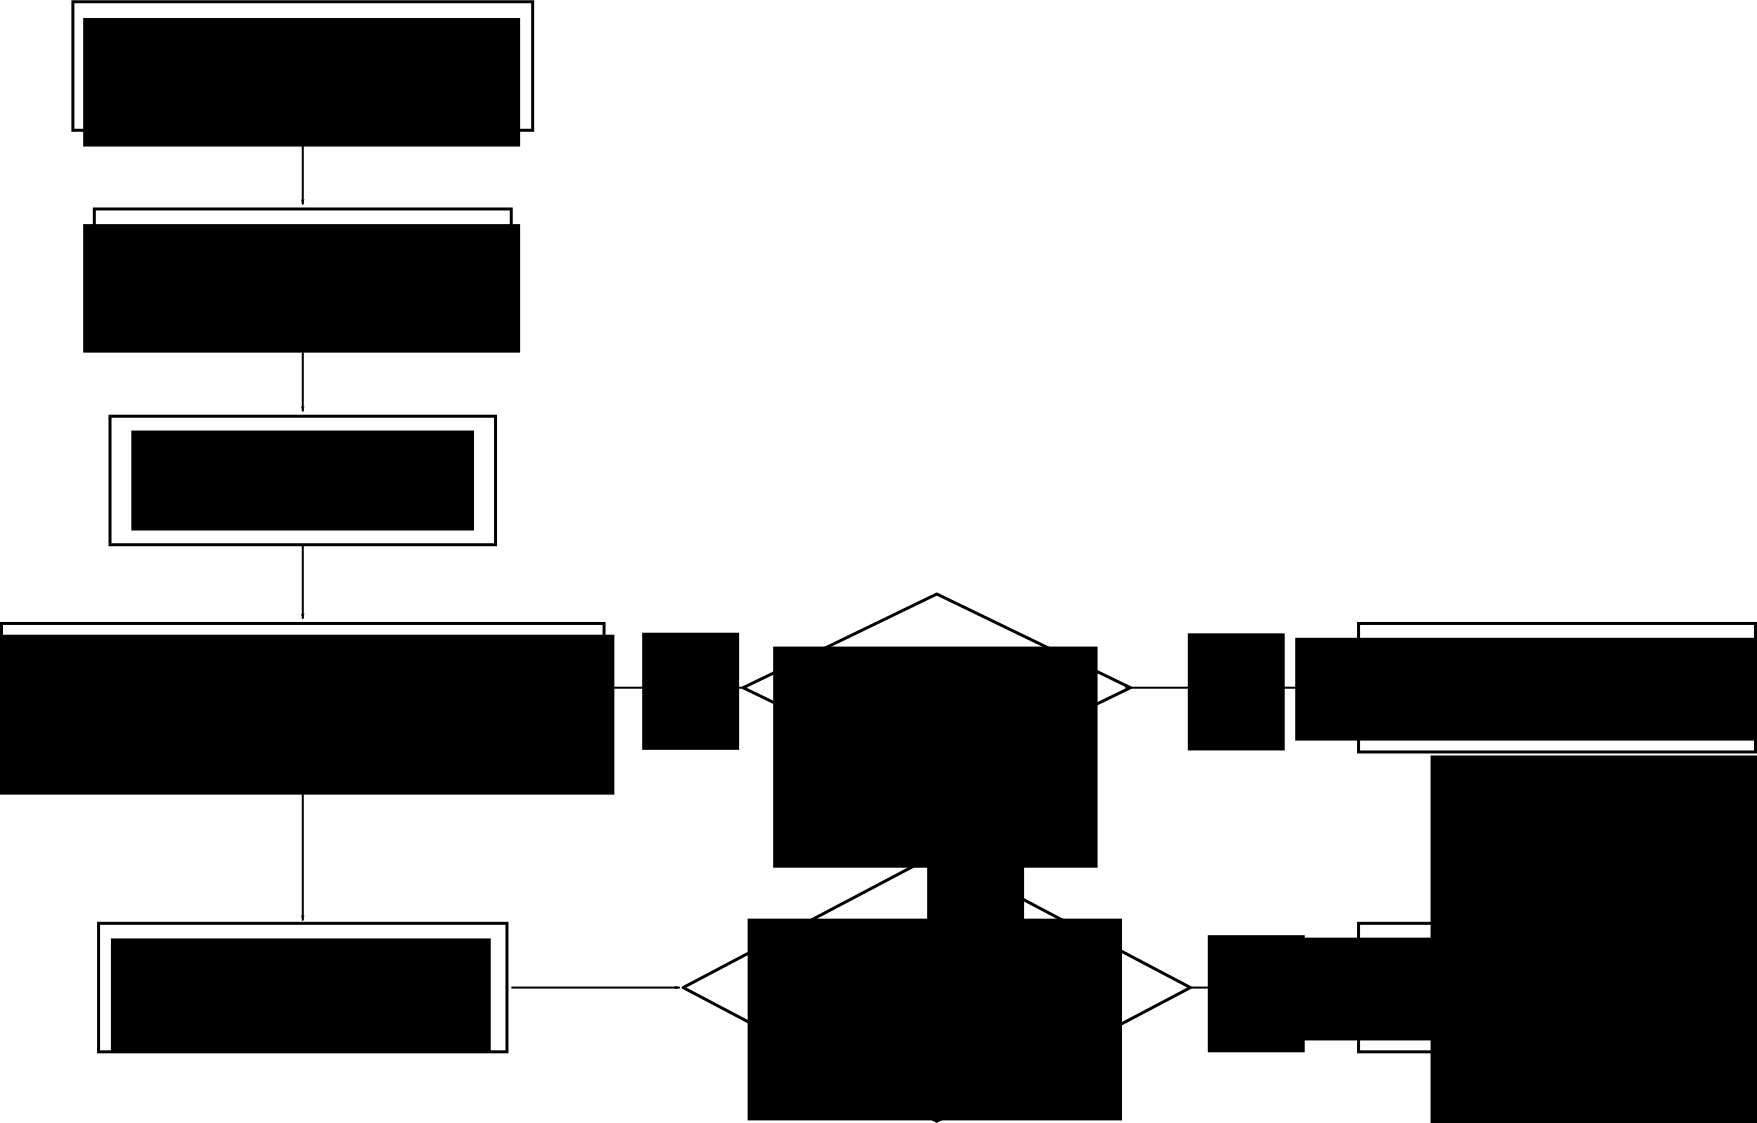
\includegraphics[width=0.85\textwidth]{\Flexion/figs/diagrama-de-flujo-parker-oldenburg.pdf}
    \caption{Diagrama de Flujo del algoritmo de inversi�n de Paker-Oldenburg implementado en Python.}
    \label{fig-diagrama-flujo-parker-oldenburg}
\end{figure}

Como entrada del programa tomamos una grilla regular de las anomal�as de Bouguer [m/s$^{2}$] en coordenadas planas, adem�s de los siguientes par�metros: espesor de corteza normal $t$, contraste de densidad de la ra�z $\Delta\rho = \rho_{m} - \rho_{c}$, orden m�ximo $N$ de la sumatoria, valor de tolerancia y un factor de corte utilizado por el filtro de Hamming.


Lo primero que realizamos es calcular el t�rmino constante a partir de la TF de las anomal�as, el cual es una cantidad invariante durante todo el proceso iterativo. Las Transformadas de Fourier y sus Antitransformadas son calculadas a lo largo de todo el proceso de inversi�n a trav�s de las funciones fftpack.fft2 y fftpack.iff2 de las librer�as SciPy (\cite{SciPy}). Mientras que los vectores de frecuencias son calculados con la funci�n fftpack.fftfreq, tambi�n de SciPy.

Luego proponemos una deflexi�n inicial, que sirve �nicamente como punto de partida para el algoritmo. En nuestro caso elegimos partir con una deflexi�n nula para todo punto de la grilla.

\subsection{C�lculo de Nueva Deflexi�n con Parker-Oldenburg}
\label{subsection-nueva-deflexion-parker-oldenburg}

En este paso obtenemos la TF de una nueva deflexi�n haciendo uso de la ecuaci�n \ref{eq-parker-oldenburg-iterativo}, tomando el t�rmino constante ya calculado y la deflexi�n obtenida en la iteraci�n anterior (en caso de ser �sta la primer iteraci�n, tomamos como deflexi�n anterior la inicialmente propuesta).

Antes de antitransformarla para obtener la nueva ra�z propiamente dicha, aplicamos el filtro de Hamming a su Transformada. Para lo cual es necesario determinar un valor para la frecuencia de corte $k_{cut}$. Como este par�metro es el que est� m�s liberado a la subjetividad del usuario, decidimos darle una interpretaci�n f�sica. Para ello propusimos que sea proporcional a la frecuencia asociada al espesor de la corteza normal.

Se sabe que una fuente localizada a una profundidad $d$ generar� efectos gravim�tricos con longitudes de onda de aproximadamente $2\pi/d$. Es por ello que al eliminar las frecuencias mayores  s�lo descartamos las contribuciones de las fuentes que est�n a menor profundidad que $d$.

Es por ello que vamos a definir al $k_{cut}$ como:
\begin{equation}
    k_{cut} = \textrm{factor de corte} \cdot \frac{\pi}{t}
\end{equation}
donde el factor de corte es el par�metro de entrada. Este valor puede variar entre 0 y 2, y aunque est� asociado con una interpretaci�n f�sica, sigue quedando sujeto a la subjetividad del usuario en funci�n del resultado que el algoritmo genere, solo que ahora contamos con una interpretaci�n del mismo.

Una vez aplicado el filtro de Hamming con la frecuencia de corte deseada, antitransformamos el resultado para obtener as� la nueva deflexi�n.


\subsection{Criterio de Interrupci�n del Algoritmo}
En algoritmos iterativos de este tipo es necesario contar con un criterio de interrupci�n que determine cu�ndo este converge o alcanza una situaci�n deseada, o bien cuando diverge.

En este caso propusimos calcular la desviaci�n est�ndar entre la deflexi�n de la iteraci�n actual con la de la anterior como: 
\begin{equation}
    \textrm{RMS} = \sqrt{ \frac{1}{N_{x}N_{y}} \sum\limits_{n=1}^{N_{x}} \sum\limits_{m=1}^{N_{y}} \big[w_{i}(x_{n}, y_{m}) - w_{i-1}(x_{n}, y_{m})\big]^{2}}
\end{equation}
donde $N_{x}$ y $N_{y}$ son la cantidad de puntos por eje que posee la grilla de valores de anomal�a de Bouguer sobre la cual trabajamos; y $w_{i}$ y $w_{i-1}$ son las ra�ces de las iteraciones actuales y anteriores, respectivamente.

En caso de que el RMS sea menor que el valor de tolerancia elegido, entonces consideramos que el algoritmo converge finalizando exitosamente y devolviendo la r�iz obtenida en est� �ltima iteraci�n. Caso contrario, verificamos que el valor de RMS no haya incrementado desde el valor que obtuvo en la iteraci�n previa. Si lo ha hecho damos por finalizado el algoritmo como no convergente, devolviendo la ra�z obtenida en la iteraci�n anterior.

Si el RMS no alcanza la tolerancia ni se incrementa desde la iteraci�n anterior, entonces procedemos a calcular una nueva ra�z como se describi� en \ref{subsection-nueva-deflexion-parker-oldenburg} y continuar iterativamente con el algoritmo.

\section{Modelo Sint�tico para Inversi�n del Moho}
Con el objetivo de corroborar el funcionamiento del algoritmo de inversi�n, aqu� proponemos un modelo sint�tico que consiste en una corteza normal de ancho $t$ y densidad $\rho_{c}=2900$kg/m$^{3}$, sobre un manto de densidad $\rho_{m}=3300$kg/m$^{3}$, la cual se deflecta como lo muestra la primer gr�fica de la Figura \ref{fig-sintetico-parker-oldenburg}. Trabajamos sobre una grilla de 400km$\times$400km con 101$\times$101 nodos.

\begin{figure}[b!]
    \centering{}
    \includegraphics[width=0.85\textwidth]{\Flexion/figs/sintetico-parker-oldenburg-perfil.pdf}
    \caption{Perfiles correspondientes a las deflexiones sint�ticas e invertida realizados en las l�neas de puntos que se ven en la Figura \ref{fig-sintetico-parker-oldenburg}.}
    \label{fig-sintetico-parker-oldenburg-perfil}
\end{figure}

Para calcular la anomal�a gravim�trica que la ra�z genera, construimos un ``mesh'' de 100$\times$100 prismas rectangulares que se extienden verticalmente desde $-t$ hasta un promedio entre las profundidades de la ra�z en los cuatro v�rtices del prisma. De esta manera generamos un conjunto de prismas que se aproximan geom�tricamente a la ra�z (ver Figura \ref{fig-sintetico-raiz-prismas}).

Haciendo uso de funciones de la librer�a Fatiando a Terra (\cite{Uieda2014}), pudimos determinar la anomal�a que genera la ra�z como la contribuci�n a la atracci�n gravitatoria que genera cada uno de los prismas. Para lo cual, la funci�n prism.gz de fatiando.gravmag hace uso de los resultados de \cite{Nagy2000} acerca del potencial gravitatorio generado por prismas. La anomal�a de Bouguer que se obtiene se puede ver en la segunda gr�fica de la Figura \ref{fig-sintetico-parker-oldenburg}.

\begin{figure}[t!]
    \centering{}
    \includegraphics[width=0.98\textwidth]{\Flexion/figs/sintetico-parker-oldenburg.png}
    \caption{Modelo Sint�tico para demostrar un ejemplo del algoritmo de Parker-Oldenburg. La primer gr�fica muestra la deflexi�n propuesta por el modelo, mientras que a su derecha se expone la anomal�a gravim�trica que ella genera (obtenida a trav�s de un modelado con prismas, ver Figura \ref{fig-sintetico-raiz-prismas}). La tercer gr�fica muestra la ra�z que se obtiene al invertir las anomal�as usando Parker-Oldenburg y la �ltima muestra la diferencia entre ambas deflexiones.}
    \label{fig-sintetico-parker-oldenburg}
\end{figure}

Luego, procedemos a invertir la anomal�a obtenida a trav�s del algoritmo implementado. Para ello consideramos un factor de corte igual a 2, las sumatorias hasta el orden 30 y el valor de tolerancia lo tomamos de 1$\cdot$10$^{-10}$m.
Despu�s de 17 iteraciones, el algoritmo converge a la ra�z que se muestra en la tercera gr�fica de la Figura \ref{fig-sintetico-parker-oldenburg}.

A modo de comparaci�n entre la ra�z sint�tica propuesta y la obtenida a trav�s del algoritmo de inversi�n; en la �ltima gr�fica de la Figura \ref{fig-sintetico-parker-oldenburg} se muestra una deflexi�n residual, es decir, la diferencia entre la invertida y la original. Y en la Figura \ref{fig-sintetico-parker-oldenburg-perfil} podemos ver el perfil de ambas deflexiones en un corte que en las Figuras \ref{fig-sintetico-parker-oldenburg} se muestra como l�neas de puntos.

Mediante este modelo sint�tico podemos ver que el algoritmo permite invertir de forma aproximada la deflexi�n de la corteza a partir de las anomal�as de Bouguer. Es interesante hacer hincapi� en dos cuestiones acerca del resultado del mismo.

La primera involucra los efectos de borde. Como se puede ver tanto en la gr�fica de la Deflexi�n Residual como en el perfil, la ra�z invertida se escapa de la original en los extremos de la grilla. Esto se debe a efectos de borde producidos por los m�todos espectrales y es algo a tener en cuenta cuando deseamos utilizar la ra�z invertida para futuros c�lculos o bien para interpretar datos. La segunda cuesti�n tiene que ver con un detalle que \cite{Braitenberg2002} ya hizo menci�n: el algoritmo de Parker-Oldenburg suele subestimar la profundidad del Moho, lo cual se traducir� luego en una sobrestimaci�n del espesor el�stico $T_{e}$.

\begin{figure}[t!]
    \centering{}
    \includegraphics[width=0.98\textwidth]{\Flexion/figs/sintetico-raiz-prismas.png}
    \caption{Conjunto de prismas utilizado para simular la deflexi�n propuesta y calcular a partir de ellos la anomal�a gravim�trica que genera.}
    \label{fig-sintetico-raiz-prismas}
\end{figure}


\section{Mejora a Parker-Oldenburg}
Con el objetivo de solucionar el problema que presenta el algoritmo de Parker-Oldenburg, aqu� proponemos una mejora al m�todo, que consiste en realizar correcciones a la deflexi�n que se obtiene calculando la anomal�a residual, es decir, la diferencia entre Bouguer y la anomal�a que la deflexi�n invertida genera.

Supongamos que hemos obtenido a partir de Parker-Oldenburg una deflexi�n que denominamos $w_{\rm PO}$ y llamo $\Delta g_{\rm PO}$ a la anomal�a que esa deflexi�n genera. Vamos a definir a la anomal�a residual como:
\begin{equation}
    \delta g = \Delta g_{bg} - \Delta g_{\rm PO}
\end{equation}

Podemos interpretar a esta anomal�a residual como la que genera el agregado o la sustracci�n de masa a $w_{PO}$, hasta que esta alcanza la ra�z objetivo $w$ (ver Figura \ref{fig-mejora-po-diagrama-deflexiones}). En ese caso, podemos hacer uso de la ecuaci�n \ref{eq-parker} de Parker:
\begin{equation}
    \mathcal{F} \big[ \delta g \big] = + 2\pi G (\rho_{m}-\rho_{c}) \,\, e^{-kt} \, \sum\limits_{n=1}^{\infty} \frac{k^{\,n-1}}{n!} \, \mathcal{F} \Big[\big\{ \underbrace{-w_{\rm PO}({\bf r})}_{\mathclap{\textrm{Superficie superior}}} \big\}^{n} - \big\{ \underbrace{-w({\bf r})}_{\mathclap{\textrm{Superficie inferior}}}\big\}^{n} \Big]
\end{equation}

\begin{figure}[t!]
    \centering{}
    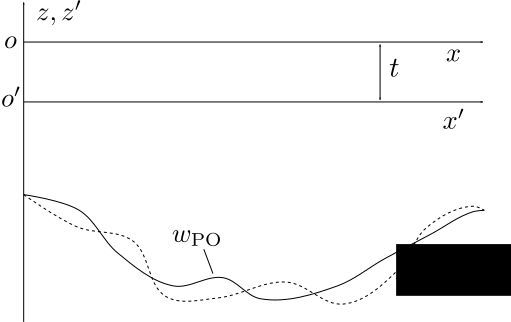
\includegraphics[width=0.65\textwidth]{\Flexion/figs/mejora-parker-oldenburg-diagrama-deflexiones.pdf}
    \caption{Esquema de la deflexi�n invertida mediante Parker-Oldenburg y la deflexi�n objetivo, es decir, la que genera fielmente la anomal�a de Bouguer.}
    \label{fig-mejora-po-diagrama-deflexiones}
\end{figure}

Reordenando la ecuaci�n anterior obtenemos la siguiente relaci�n:
\begin{equation}
    \mathcal{F} \big[ w({\bf r}) - w_{\rm PO}({\bf r}) \big] = - \frac{\mathcal{F}[\,\delta g\,]\,e^{kt}}{2\pi G(\rho_{m}-\rho_{c})} \,\, - \,\, \sum\limits_{n=2}^{\infty} \frac{(-1)^{n} k^{\,n-1}}{n!} \, \mathcal{F} \big[ w^{n}({\bf r}) - w_{\rm PO}^{n} ({\bf r}) \big]
\end{equation}

A partir de ella podemos proponer un m�todo iterativo similar al de Parker-Oldenburg:
\begin{equation}
    \mathcal{F} \big[ w_{i} - w_{\rm PO} \big] = - \frac{\mathcal{F}[\,\delta g\,]\,e^{kt}}{2\pi G(\rho_{m}-\rho_{c})} \,\, - \,\, \sum\limits_{n=2}^{N} \frac{(-1)^{n} k^{\,n-1}}{n!} \, \mathcal{F} \big[ w_{i-1}^{n} - w_{\rm PO}^{n} \big]
\end{equation}

De esta manera podemos obtener una nueva deflexi�n que ajuste de forma m�s precisa la anomal�a residual. Proponemos realizar este proceso iterativamente: utilizamos al principio la deflexi�n que se obtiene por Parker-Oldenburg para calcular una $w^{1}$; esta tomar� luego el lugar de la primera; computamos la anomal�a residual que esta nueva ra�z genera y mediante un m�todo similar a Parker-Oldenburg obtenemos la deflexi�n $w^{2}$. 

Podemos resumir �ste m�todo en la siguiente ecuaci�n, donde $i$ barre iteraciones del simil Parker-Oldenburg, mientras que $j$ barre las iteraciones en las que recalculamos la anomal�a residual.
\begin{equation}
    \boxed{ \mathcal{F} \big[ w^{\,j}_{i} - w^{\,j-1} \big] = - \frac{\mathcal{F}[\,\delta g^{\,j-1}\,]\,e^{kt}}{2\pi G(\rho_{m}-\rho_{c})} \,\, - \,\, \sum\limits_{n=2}^{N} \frac{(-1)^{n} k^{\,n-1}}{n!} \, \mathcal{F} \big[ \{ w^{\,j}_{i-1} \}^{n} - \{ w^{\,j-1} \}^{n} \big] }
    \label{eq-parker-oldenburg-mejorado}
\end{equation}
\begin{equation}
    \textrm{con}\quad\delta g^{\,j-1} = \Delta g_{bg} - \Delta g^{\,j-1}
\end{equation}

\begin{figure}[t!]
    \centering{}
    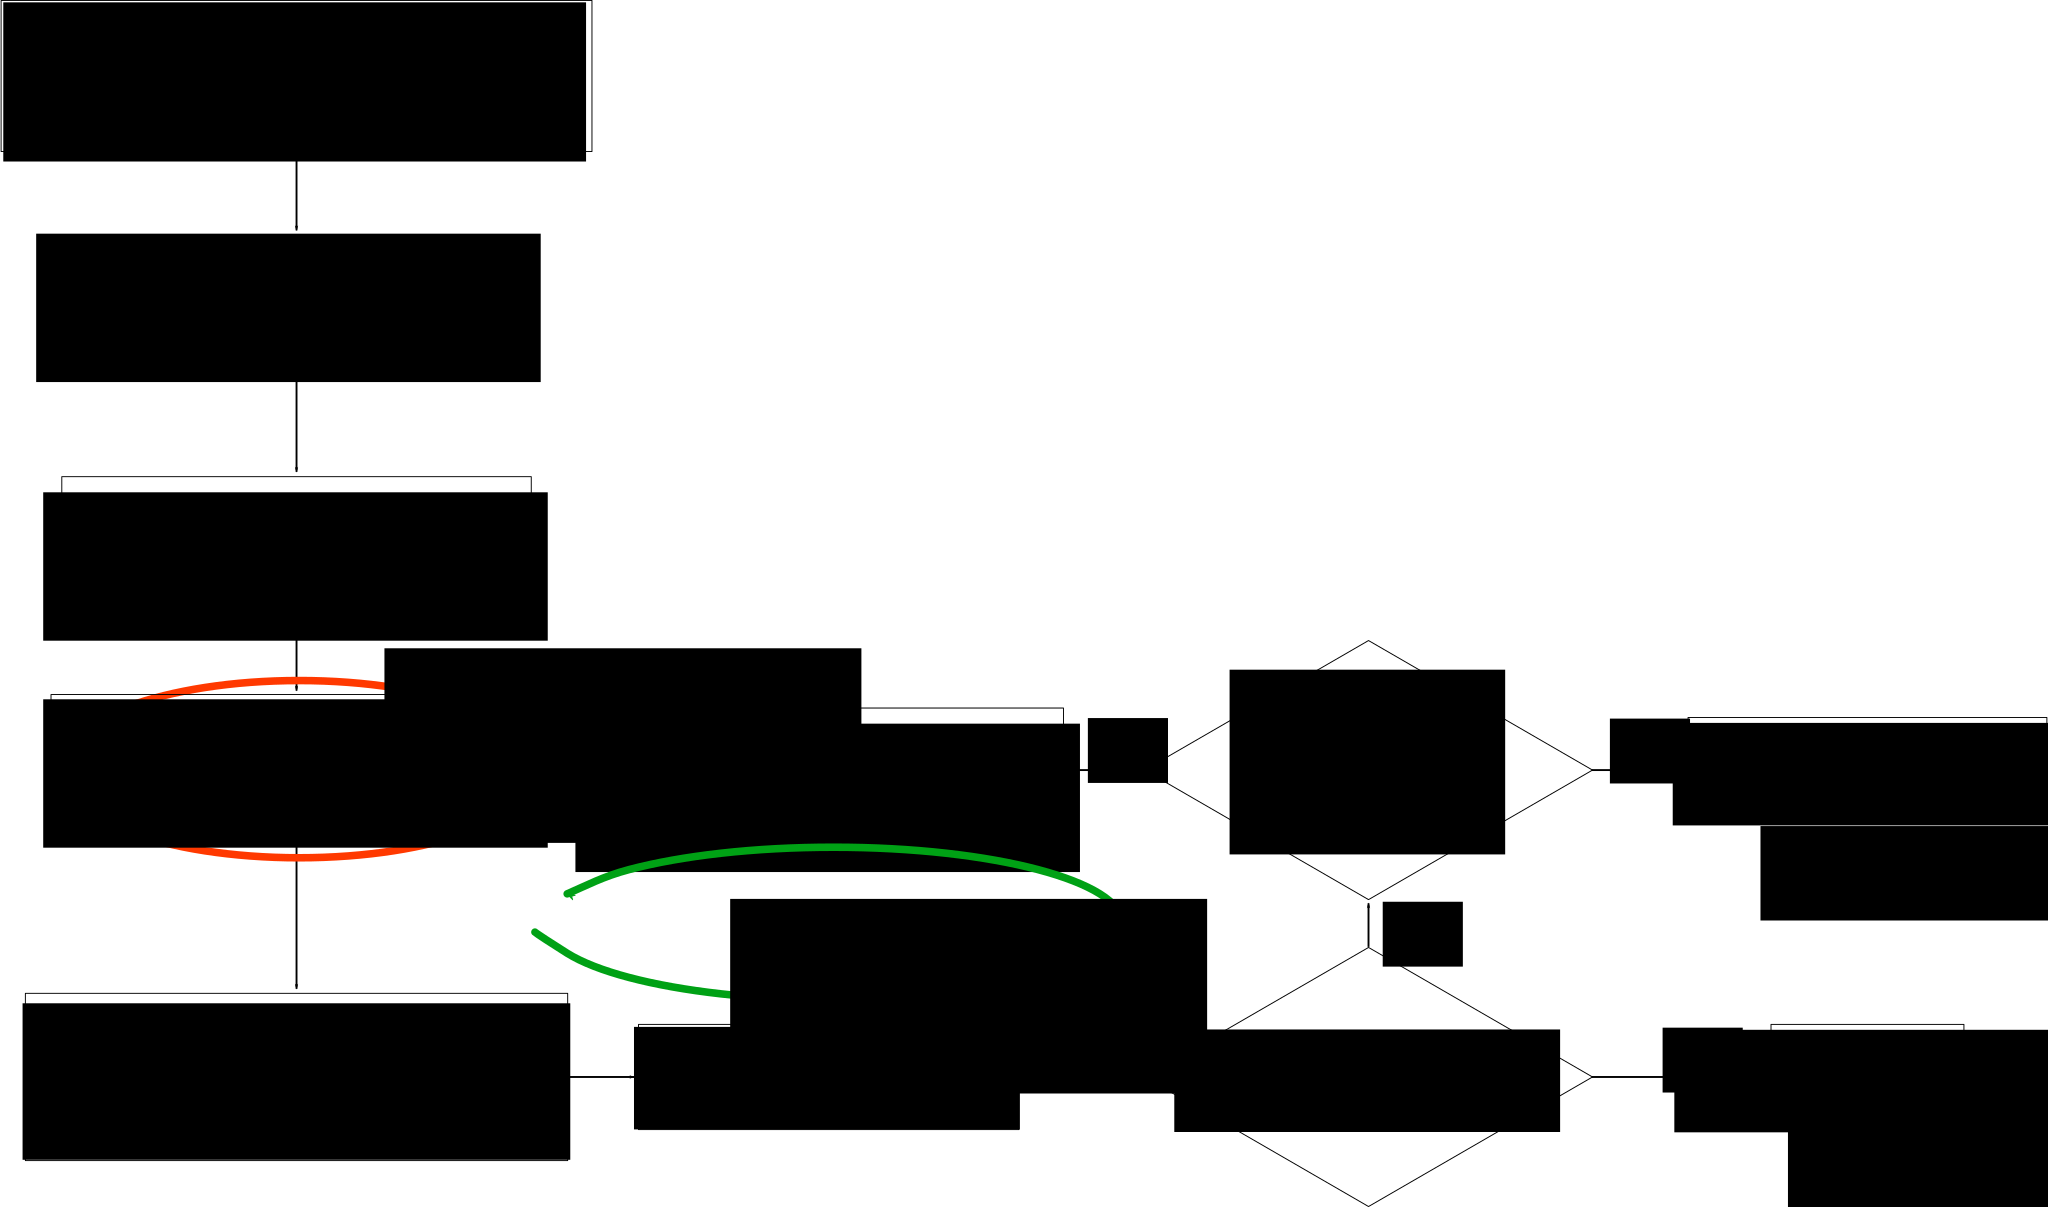
\includegraphics[width=0.98\textwidth]{\Flexion/figs/mejora-parker-oldenburg-diagrama-de-flujo.pdf}
    \caption{Diagrama de Flujo del algoritmo de mejora a Parker-Oldenburg.}
    \label{fig-mejora-po-diagrama-de-flujo}
\end{figure}

En la Figura \ref{fig-mejora-po-diagrama-de-flujo} se muestra el diagrama de flujo del algoritmo en cuesti�n. All� se puede ver que el criterio de interrupci�n utilizado es similar al de Parker-Oldenburg, solo que ahora comparamos la anomal�a que genera cada deflexi�n $w^{\,j}$ con la anomal�a de Bouguer original. Si el RMS que se obtiene es menor que a un valor de tolerancia damos por finalizado con �xito al m�todo.

En esta mejora solo utilizamos un filtro pasabajos dentro del simil Parker-Oldenburg. Por lo tanto el RMS entre la anomal�a de Bouguer y la que genera cada deflexi�n $w^{\,j}$ puede ser alto, ya que la primera poseer� componentes de altas frecuencias que la �ltima no. Esto debe tenerse en cuenta a la hora de definir la tolerancia, o bien, filtrar la anomal�a de Bouguer antes de introducirla en el algoritmo.

Los c�lculos de la anomal�a gravitatoria que cada deflexi�n $w^{\,j}$ genera son realizados al igual que en el �ltimo modelo sint�tico: aproximando la ra�z por prismas rectangulares y obteniendo su efecto gravitatorio, haciendo uso de la funci�n prism.gz de fatiando.gravmag, disponible a trav�s de la librer�a Fatiando a Terra (\cite{Uieda2014}).

La desventaja que posee este m�todo es el tiempo de c�mputo. El proceso de calcular la anomal�a que genera la deflexi�n en cada iteraci�n $j$ requiere un tiempo de procesamiento elevado en comparaci�n con los c�lculos espectrales que se realizan con mucha velcidad. Adem�s, a medida que la grilla aumenta en ancho, la cantidad de prismas necesarios para modelizar la ra�z aumenta en potencia de 2, como tambi�n lo hace el tiempo de c�mputo. Es por ello que antes de intentar un c�lculo semejante es necesario analizar nuestra grilla de trabajo y evaluar tanto su extensi�n como su resoluci�n.

\newpage
\sectionmark{Modelo Sint�tico con Nuevo M�todo}
\section[Modelo Sint�tico para Inversi�n del Moho con Mejora a\\Parker-Oldenburg]{Modelo Sint�tico para Inversi�n del Moho con Mejora a Parker-Oldenburg}


Partiendo de la deflexi�n obtenida por Parker-Oldenburg en el ejemplo de la Figura \ref{fig-sintetico-parker-oldenburg} aplicamos el m�todo descripto en los �ltimos p�rrafos para obtener una deflexi�n que ajuste mejor a la original.

Para ello extendimos las sumatorias de la ecuaci�n \ref{eq-parker-oldenburg-mejorado} hasta orden 15, utilizamos un factor de corte igual a 1 para el filtro pasabajos y los valores de tolerancia usados fueron de 10$^{-3}$m para el simil Parker-Oldenburg y 10$^{-8}$m/s$^{2}$ para el RMS entre la anomal�a de Bouguer y la anomal�a generada por cada deflexi�n $w^{\,j}$.

En la Figura \ref{fig-sintetico-mejora-parker-oldenburg} se muestran las gr�ficas de la deflexi�n sint�tica (la misma que la del modelo sint�tico previo) y la invertida a trav�s del nuevo m�todo. Adem�s, se exponen las deflexi�n y anomal�a residuales. A simple vista podemos observar que bajaron considerablemente los valores de la deflexi�n residual y que ahora la ra�z no est� subestimada.

Para visualizar mejor el ajuste de la ra�z, en la Figura \ref{fig-sintetico-mejora-perfil} se puede ver los perfiles de las deflexiones original e invertida, respectivamente; en un perfil delimitado por las lineas de puntos de la Figura \ref{fig-sintetico-mejora-parker-oldenburg}. En ella se puede apreciar que el ajuste es mucho m�s preciso que haciendo uso de Parker-Oldenburg. Sin embargo, continuamos teniendo los efectos de borde, por ende debemos seguir teni�ndolos en cuenta a la hora de construir nuestras grillas de inversi�n.

\begin{figure}[h!]
    \centering{}
    \includegraphics[width=0.85\textwidth]{\Flexion/figs/sintetico-mejora-perfil.pdf}
    \caption{Perfiles correspondientes a las deflexiones sint�tica e invertida realizados en las l�neas de puntos que se ven en la Figura \ref{fig-sintetico-mejora-parker-oldenburg}.}
    \label{fig-sintetico-mejora-perfil}
\end{figure}


\newpage
\begin{figure}[h!]
    \centering{}
    \includegraphics[width=0.98\textwidth]{\Flexion/figs/sintetico-mejora-parker-oldenburg.png}
    \caption{Modelo Sint�tico para demostrar un ejemplo de la mejora al algoritmo de Parker-Oldenburg. La primer gr�fica muestra la deflexi�n propuesta por el modelo, mientras que a su derecha se expone la deflexi�n que se obtiene de dicho m�todo. Las �ltimas dos muestran la deflexi�n y anomal�a residuales, respectivamente; es decir, las diferencias entre las deflexiones y anomal�as gravitatorias originales y las generadas por el m�todo de inversi�n.}
    \label{fig-sintetico-mejora-parker-oldenburg}
\end{figure}
$\ $



\prechapterpage
\chapter{Determinaci�n del Espesor El�stico}

Siendo capaces de invertir el Moho a trav�s de las anomal�as de Bouguer, estamos en condiciones de proceder a la determinaci�n del espesor el�stico de la corteza. Como hemos dicho anteriormente, lo haremos calculando cu�l es el valor de $T_{e}$ que mejor ajusta en la ecuaci�n \ref{eq-deflexion-topografia-freq}, haciendo uso de la topograf�a $h({\bf r})$ y la deflexi�n invertida $w({\bf r})$.

Para lo cual es necesario suponer que el espesor el�stico es constante en toda la zona de estudio, lo cual no suele suceder en situaciones reales. Solucionaremos esto trabajando con ventanas peque�as, dentro de las cuales supondremos que dicha hip�tesis es v�lida.

Sin embargo, al desechar los datos de topograf�a y deflexi�n exteriores a la ventana, caemos en el error de calcular una deflexi�n local, sin importarnos qu� cargas tenemos alrededor de dicha ventana ni c�mo deflectan regionalmente la peque�a zona que estamos analizando.

Para evitarlo, aqu� proponemos obtener una deflexi�n de prueba por cada valor de $T_{e}$ posible, haciendo uso de la ecuaci�n \ref{eq-deflexion-topografia-freq} y considerando la carga topogr�fica de toda la zona de estudio; luego comparar estas deflexiones de prueba con la invertida solo en la ventana en la que estamos parados. Tomando finalmente como el $T_{e}$ �ptimo, aquel que minimiza la desviaci�n est�ndar entre las subgrillas de las deflexiones de prueba e invertida.

Para hacerlo hemos desarrollado una simple interfaz que permite seleccionar ventanas modificando su posici�n y tama�o; adem�s de un rango de valores de espesor el�stico posibles, dentro de los cuales se estima que se encuentra el caracter�stico de la ventana en cuesti�n.

El c�lculo del $T_{e}$ �ptimo lo llevamos a cabo obteniendo una deflexi�n de prueba para cada valor de espesor el�stico determinado y calculando la desviaci�n est�ndar entre cada una de ellas y la deflexi�n invertida anteriormente. Con estos valores generamos una gr�fica de RMS vs $T_{e}$, tomando como $T_{e}$ �ptimo aquel que minimiza el RMS. Con dicho valor graficamos en �reas m�s peque�as los valores de deflexi�n invertida y la deflexi�n �ptima dentro de la ventana seleccionada. En la Figura \ref{fig-flex-y-lito-captura1} se puede ver la interfaz siendo utilizada sobre una zona de estudio como ejemplo.

Una vez obtenido el $T_{e}$ que mejor ajusta en la ventana seleccionada, asociaremos al centro de la misma dicho valor de espesor el�stico. Repitiendo el proceso para un n�mero grande de ventanas obtendremos un scatter de puntos con valores de $T_{e}$ diversos. Si la densidad de puntos es suficiente, podemos realizar una interpolaci�n para obtener una grilla de valores de espesor el�stico en nuestra zona de estudio.

\begin{figure}[t!]
    \centering{}
    \includegraphics[width=0.98\textwidth]{\Flexion/figs/flex-y-lito-captura1.png}
    \caption{Interfaz gr�fica para la determinaci�n del espesor el�stico por ventanas. El primer gr�fico muestra la carta topogr�fica de la zona de estudio, a su derecha encontramos la deflexi�n previamente invertida. En ellas podemos seleccionar la ventana que deseamos analizar, pudiendo modificar su posici�n y tama�o. Una vez elegida, le ordenamos que construya la gr�fica superior derecha que contiene valores de RMS entre las ventanas de la deflexi�n invertida y las deflexiones de prueba obtenidas para cada valor de $T_{e}$ (entre 0 y 50km, en este caso). Sobre ella se muestra el valor de $T_{e}$ que minimiza dicha curva y por debajo se exponen las deflexiones invertida y �ptima s�lo en las ventanas seleccionadas.}
    \label{fig-flex-y-lito-captura1}
\end{figure}

\section[Deflexi�n de Placa Delgada con Espesor El�stico Variable]{Deflexi�n de Placa Delgada con Espesor \\El�stico Variable}
\sectionmark{Deflexi�n con Espesor El�stico Variable}
La ecuaci�n diferencial \ref{eq-garcia} determina la deflexi�n de una placa con rigidez flexural variable $D(x,y)$ a partir de las cargas topogr�ficas. Es interesante obtener 
esta deflexi�n a partir de la grilla $D(x,y)$ obtenida.

\cite{Garcia2014} proponen un algoritmo iterativo para resolver dicha ecuaci�n. Para realizarlo consideran que $D(x,y)$ var�a suavemente y lo separan entre una deflexi�n constante $D_{0}$ y una variable $D'(x,y)$:
\begin{equation}
    D(x,y)= D_{0} + D'(x,y)
\end{equation}

Definen como $w_{0}(x,y)$ a la deflexi�n que presenta una placa el�stica con la rigidez flexural constante $D_{0}$, determinada por la ecuaci�n \ref{eq-deflexion-topografia-freq}; y $w(x,y)$ a la deflexi�n de la placa con rigidez variable $D(x,y)$. El m�todo iterativo que desarrollaron permite obtener la Transformada de Fourier de $w(x,y)$ de la siguiente manera:
\begin{multline}
    \mathcal{F} \big[\, w_{i} \,\big] = \mathcal{F} \big[\, w_{0} \,\big] \,-\, \frac{\Phi_{e}(k)}{(\rho_{m}-\rho_{c})g} \, \mathcal{F} \Bigg\{ \nabla^{2} \left[ D'\, \nabla^{2} w_{i-1} \right] \,- \\
    -\, (1-\nu) \left[ \frac{\partial^{2} D'}{\partial x^{2}}  \frac{\partial^{2} w_{i-1}}{\partial y^{2}} - 2 \frac{\partial^{2} D'}{\partial x \partial y} \frac{\partial^{2} w_{i-1}}{\partial x \partial y}  + \frac{\partial^{2} D'}{\partial y^{2}}  \frac{\partial^{2} w_{i-1}}{\partial x^{2}} \right] \Bigg\}
\end{multline}
donde $\rho_{m}$ y $\rho_{c}$ son las densidades del manto y la corteza, respectivamente; $\Phi_{e}(k)$ es el filtro pasabajos definido en la ecuaci�n \ref{eq-filtro-phi} usando la rigidez flexural constante $D_{0}$; $\nu$ el m�dulo de Poisson y $w_{i}\equiv w_{i}(x,y)$ es la deflexi�n obtenida en la $i$-�sima iteraci�n.
\begin{figure}[b!]
    \centering{}
    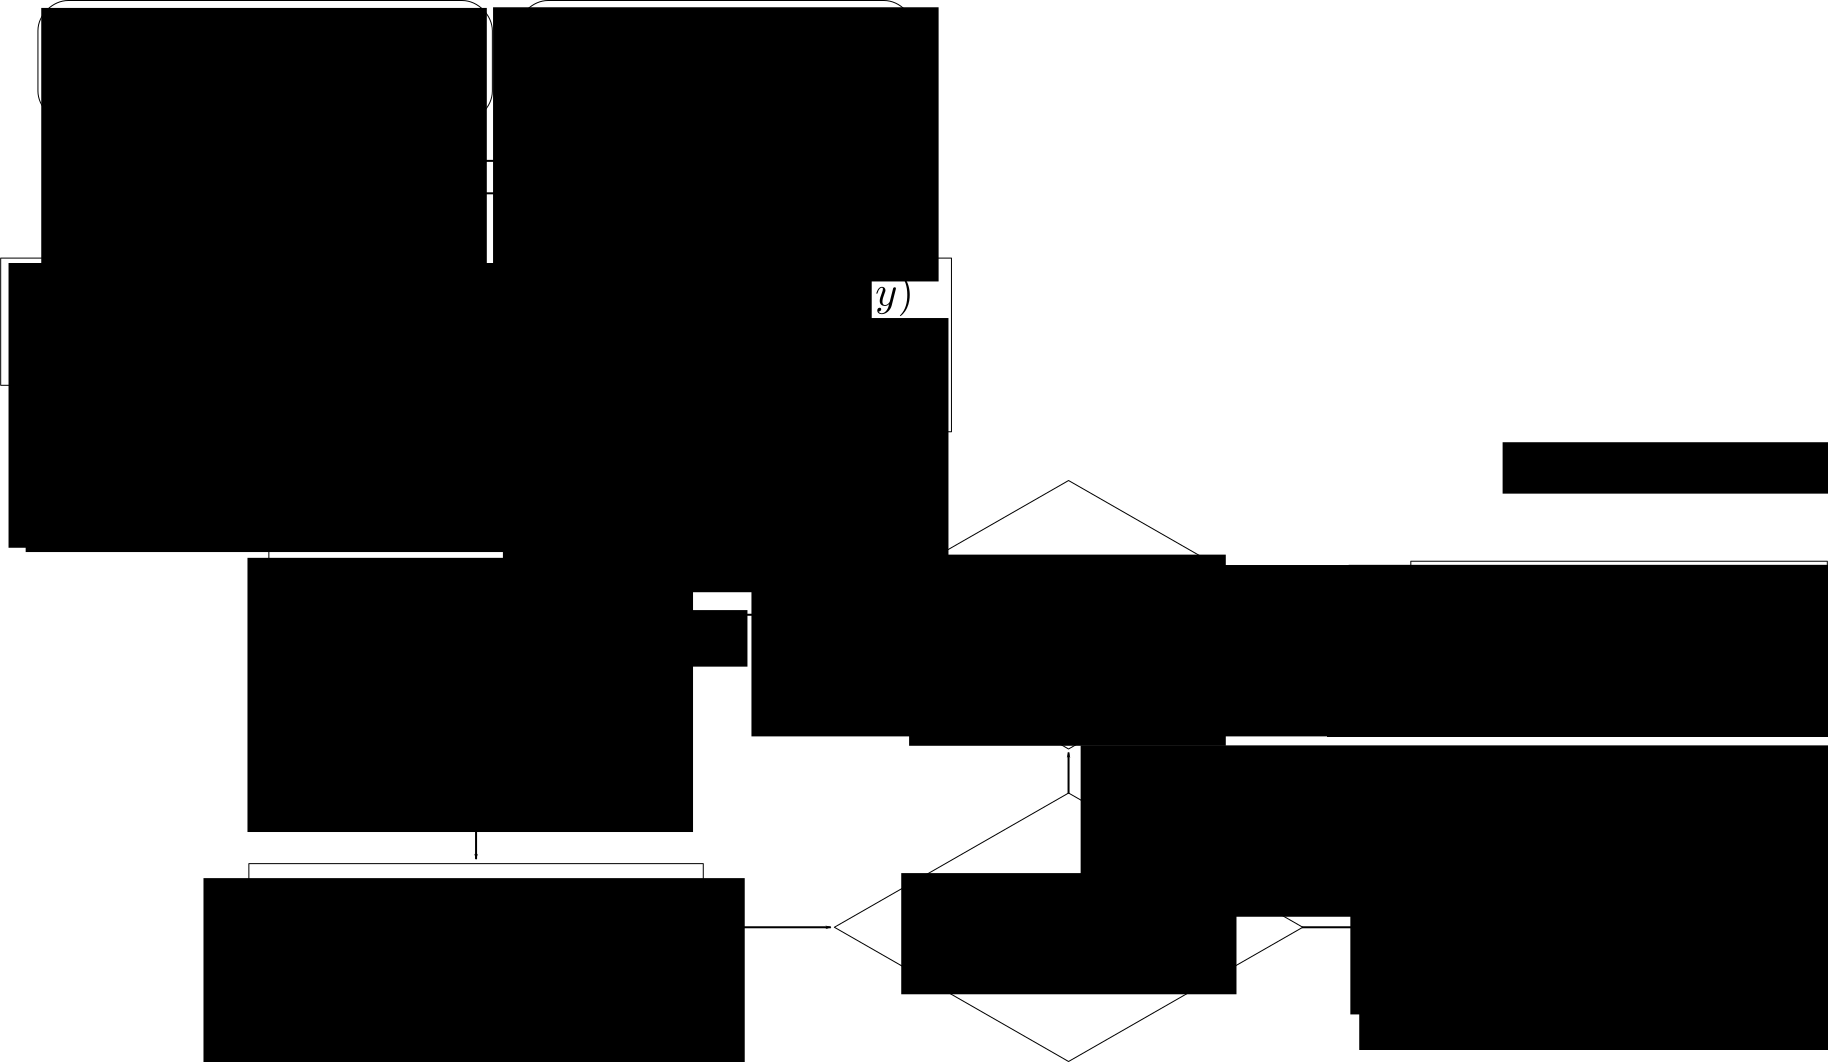
\includegraphics[width=0.98\textwidth]{\Flexion/figs/garcia-diagrama-de-flujo.pdf}
    \caption{Diagrama de Flujo del algoritmo de \cite{Garcia2014} para resoluci�n de la ecuaci�n diferencial que rige la deflexi�n de una placa delgada con rigidez flexural variable $D(x,y)$.}
    \label{fig-garcia-diagrama-de-flujo}
\end{figure}

Siguiendo las indicaciones de los autores, hemos implementado este m�todo en lenguaje Python. Las tres derivadas parciales de $D'$ pueden calcularse al incio ya que no var�an iteraci�n a iteraci�n, como s� lo hacen las derivadas de la deflexi�n $w_{i-1}$. Todas las derivaciones son realizadas espectralmente ya que es la forma m�s precisa y eficiente de obtener la derivada de valores discretos (\cite{Garcia2014}). 
\begin{equation}
\begin{gathered}
    \mathcal{F} \Big[\, \frac{\partial^{2} f }{\partial x^{2}} \,\Big] =  - \, k_{x}^{2} \, \mathcal{F} \big[\, f \,\big] \quad ,\quad \mathcal{F} \Big[\, \frac{\partial^{2} f}{\partial y^{2}} \,\Big] =  - \, k_{y}^{2} \, \mathcal{F} \big[\, f \,\big]\\
    \mathcal{F} \Big[\, \frac{\partial^{2} f}{\partial x \partial y} \,\Big] =  - \, k_{x}\,k_{y} \, \mathcal{F} \big[\, f \,\big]
\end{gathered}
\end{equation}

Las derivadas obtenidas mediante diferencias finitas amplifican las componentes de ruido, generando resultados no deseados. Para evitar esto al calcular las derivadas espectralmente; hemos filtrado las bajas frecuencias de las funciones a derivar con filtros de Hamming, usando como frecuencia de corte la frecuencia de Nyquist: $k_{cut}=\pi/dx$, donde $dx$ es la distancia entre primeros vecinos de la grilla $x,y$.

Adem�s, \cite{Garcia2014} aconsejan extender la grilla en los extremos, colocando alg�n valor constante de espesor el�stico, para evitar los efectos de borde que su m�todo introduce.

En la Figura \ref{fig-garcia-diagrama-de-flujo} se muestra un diagrama de flujo del algoritmo implementado. La utilizaci�n de los filtros pasabajos no se muestra, pero se da por entendido que est�n incluidas en los c�lculos de las derivadas tanto de $D'(x,y)$ como de cada deflexi�n $w_{i}(x,y)$.

Es interesante, luego de haber obtenido esta nueva deflexi�n, compararla con la que se calcul� a trav�s de la inversi�n de la anomal�a de Bouguer. Incluso calcular la anomal�a que genera y determinar la residual.


\section{Resumen del M�todo Completo}
Agrupemos las ideas centrales de los �ltimos cap�tulos, con el fin de ordenar los procesos necesarios para determinar el Espesor El�stico de una regi�n de inter�s.

\begin{figure}[b!]
    \centering{}
    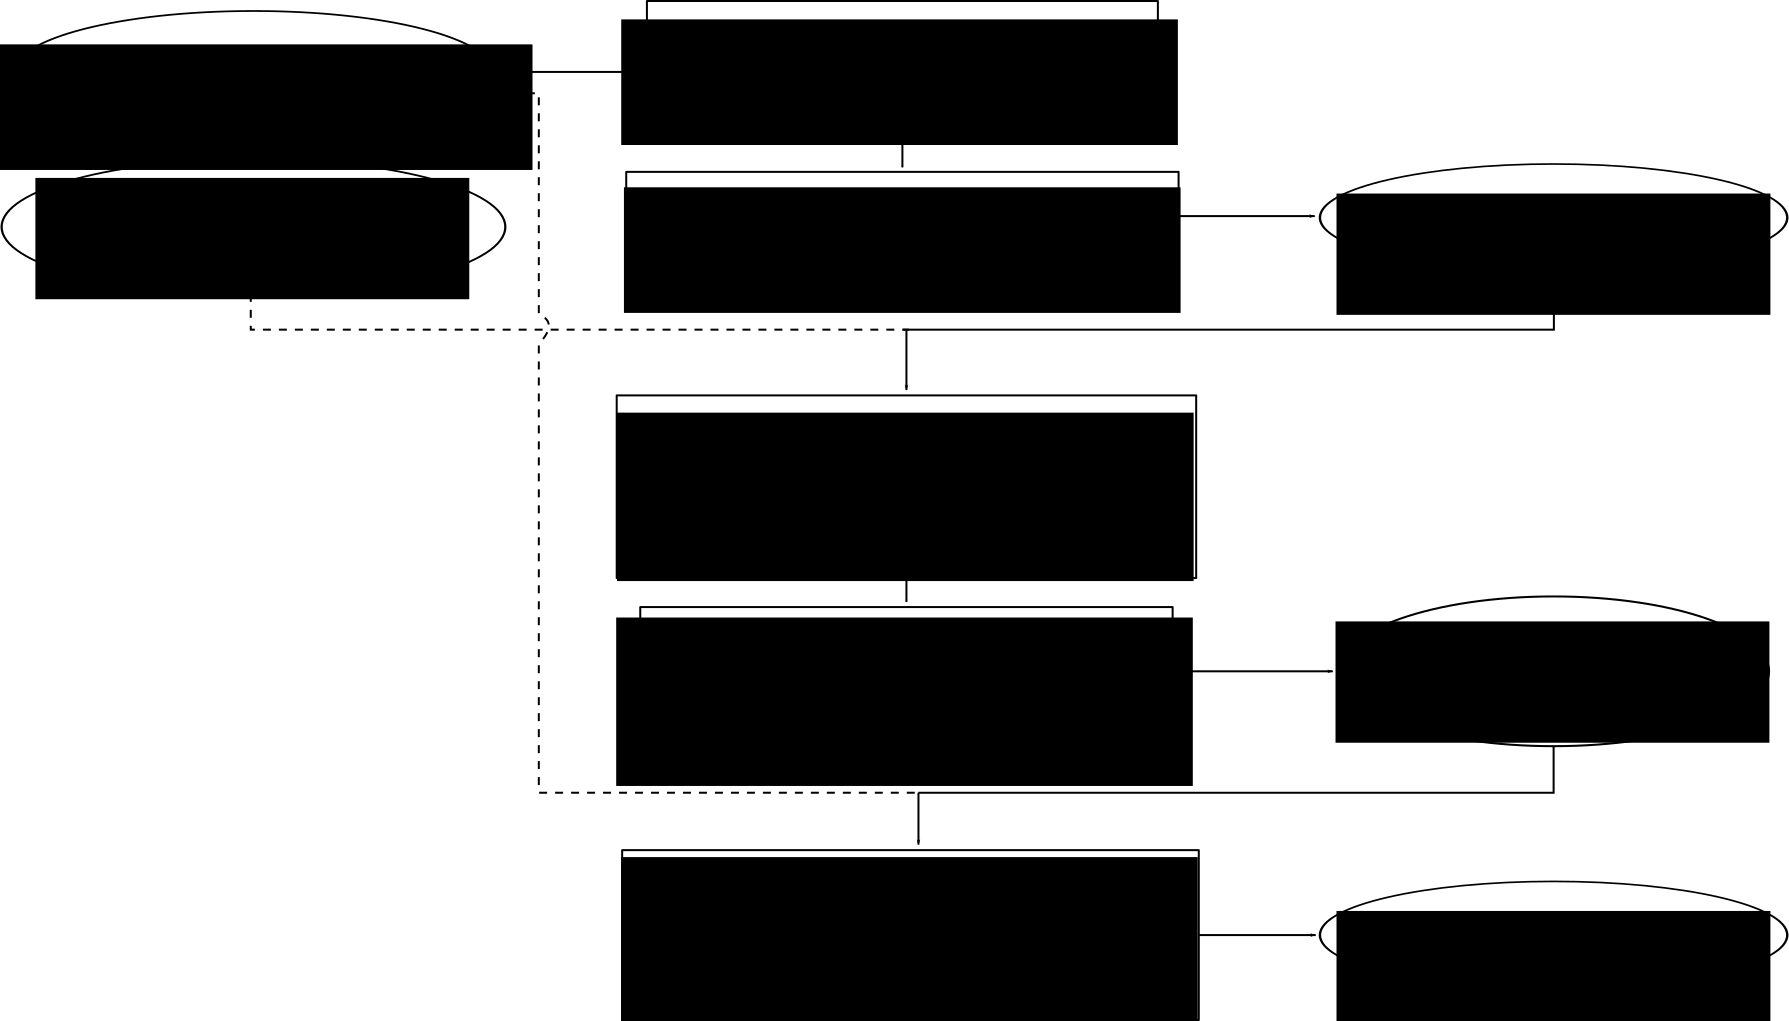
\includegraphics[width=0.9\textwidth]{\Flexion/figs/diagrama-de-flujo-metodo-completo.pdf}
    \caption{Diagrama de Flujo del m�todo completo para la determinaci�n del Espesor El�stico de la corteza terrestre.}
    \label{fig-diagrama-de-flujo-metodo-completo}
\end{figure}

Debemos partir desde la construcci�n de grillas regulares de topograf�a y anomal�as de Bouguer de nuestra zona de estudio. Las mismas deben estar en coordenadas planas, requisito necesario para que las Transformadas de Fourier trabajen con frecuencias en unidades de la inversa del metro.

El modelo de lit�sfera que proponemos est� constituido por una corteza normal de ancho $t$ y densidad $\rho_{c}$ que descansa sobre un manto no viscoso de densidad $\rho_{m}$. Consideramos que sobre dicha corteza se coloca una carga topogr�fica de densidad $\rho_{t}$ la cual produce una deflexi�n de la primera, generando una ra�z que posee la misma densidad $\rho_{c}$.

El primer paso consiste en obtener dicha deflexi�n mediante la inversi�n de las anomal�as de Bouguer. Lo hacemos aplicando primero el algoritmo de Parker-Oldenburg y luego la mejora que presentamos en este trabajo.

En segundo lugar determinaremos el espesor el�stico en la zona de estudio utilizando la grilla de topograf�a; mediante el uso de ventanas peque�as, en las cuales suponemos que el $T_{e}$ se mantiene constante. Para lograrlo se implement� una simple interfaz gr�fica que facilita la selecci�n de las ventanas, la visualizaci�n y la escritura de los datos que se van construyendo. Cada valor de espesor el�stico es asociado al centro de su respectiva ventana.

Una vez que contamos con una densidad de puntos de $T_{e}$ considerable, procedemos a interpolarlos sobre una grilla regular; para luego aplicar el algoritmo propuesto por \cite{Garcia2014} para la determinaci�n de una deflexi�n flexural a partir de la grilla de espesor el�stico y la carga topogr�fica.

En la Figura \ref{fig-diagrama-de-flujo-metodo-completo} se muestra un diagrama de flujo que sintetiza el m�todo completo para la determinaci�n del espesor el�stico.



%~ \section[Sint�tico para Determinaci�n de Espesor El�stico]{Sint�tico para Determinaci�n de Espesor\\El�stico}
\sectionmark{Modelo Sint�tico para Determinaci�n de $T_{\lowercase{e}}$}
\section{Modelo Sint�tico para Determinaci�n de Espesor El�stico}
\sectionmark{Modelo Sint�tico para Determinaci�n de $T_{\lowercase{e}}$}
Con el objetivo de corroborar el funcionamiento del m�todo global, construimos un modelo sint�tico a partir de una grilla de topograf�a arbitraria de 61$\times$61 nodos, como se ve en la Figura \ref{fig-sintetico-completo}a. Consideramos una corteza normal de ancho $t=35$km y densidades de topograf�a, corteza y manto $\rho_{t}=2670$kg/m$^{3}$, $\rho_{t}=2900$kg/m$^{3}$ y $\rho_{t}=3300$kg/m$^{3}$, respectivamente. Propusimos un espesor el�stico que aumenta linealmente en $y$ (ver Figura \ref{fig-sintetico-completo}b); y utilizando el algoritmo de \cite{Garcia2014} obtuvimos la deflexi�n que la carga topogr�fica genera (Figura \ref{fig-sintetico-completo}c); para luego calcular la anomal�a que produce mediante el modelado con prismas (Figura \ref{fig-sintetico-completo}d). De esta forma tenemos las dos grillas de entrada para nuestro m�todo: la topograf�a y la anomal�a de Bouguer.

Lo primero que hacemos es invertir la anomal�a para obtener el Moho, aplicando Parker-Oldenburg y la mejora propuesta en este trabajo. En el primero utilizamos un factor de corte igual a 1, extendimos el orden de las sumatorias hasta 15 y el valor de tolerancia lo fijamos en 10$^{-8}$m. Para la mejora aplicamos los mismos par�metros m�s un valor de tolerancia de 10$^{-8}$m/s$^{2}$. La deflexi�n resultante de la inversi�n se puede ver en la Figura \ref{fig-sintetico-completo-1}a, y compar�ndolo con la deflexi�n original o sint�tica de la Figura \ref{fig-sintetico-completo}c vemos que ambas ajustan satisfactoriamente. En la Figura \ref{fig-sintetico-completo-1}b se muestra la anomal�a residual, es decir, la diferencia entre la anomal�a de Bouguer sint�tica (Fig. \ref{fig-sintetico-completo}d) y la que genera la ra�z invertida. Estas discrepancias no superan el $0,1\%$ de la anomal�a original, reforzando a�n m�s la validez de la deflexi�n obtenida.

En segundo lugar calculamos valores de espesor el�stico usando el software de ventanas interactivas. En su mayor�a utilizamos ventanas de 20km de ancho sobre 155 puntos distribuidos en toda la regi�n, a excepci�n de los extremos de la grilla donde suponemos la presencia de efectos de borde. Finalmente interpolamos este scatter sobre la grilla regular con la que venimos trabajando. El resultado se puede apreciar en la Figura \ref{fig-sintetico-completo-1}c.

A simple vista, la comparaci�n entre la grilla de Espesor El�stico obtenida con la original parece ser desalentadora, sin embargo, al calcular la diferencia entre ambas (Figura \ref{fig-sintetico-completo-1}d) observamos que en los puntos m�s interiores las discrepancias no superan los 600m, representando no m�s del $7\%$ de error. Las mayores diferencias se dan cerca de los extremos, donde llegan hasta los 2km, alrededor de un $20\%$ de error. Por lo tanto, podemos concluir que el modelo sint�tico se muestra exitoso en la determinaci�n del Espesor El�stico con un grado de confiabilidad del $10\%$ en los puntos interiores de la grilla de trabajo. Se debe prestar especial atenci�n a la hora de construir esta �ltima, con el fin de centrar nuestra zona de estudio dejando un lugar amplio en los extremos; donde probablemente existan efectos de borde que se ver�n arrastrados a lo largo de todo el c�lculo del $T_{e}$.


\begin{figure}[b!]
    \centering{}
    \includegraphics[width=0.95\textwidth]{\Flexion/figs/sintetico-completo.jpg}
    \caption{Grillas con los datos sint�ticos del modelo construido para la determinaci�n del espesor el�stico. En $a$ y $b$ podemos ver la topograf�a y el espesor el�stico propuesto, respectivamente; mientras que en $c$ y $d$ podemos observar la deflexi�n de la placa generada por la carga topogr�fica y la anomal�a que la misma produce, respectivamente. }
    \label{fig-sintetico-completo}
\end{figure}


Finalmente aplicamos el algoritmo de \cite{Garcia2014} para obtener la deflexi�n flexural, es decir, la ra�z que se genera debido a la carga topogr�fica si �sta posee el espesor el�stico obtenido. El resultado puede verse en la Figura \ref{fig-sintetico-completo-1}e, y en la Figura \ref{fig-sintetico-completo-1}f vemos la diferencia entre la deflexi�n sint�tica y esta �ltima. En ella podemos ver que las diferencias en los puntos interiores no superan los 200m, es decir que la discrepancia no representa m�s que el 10$\%$ de los valores de deflexi�n; manteniendo el grado de confiabilidad que establecimos en el p�rrafo anterior.


\begin{figure}[b!]
    \centering{}
    \includegraphics[width=0.95\textwidth]{\Flexion/figs/sintetico-completo-1.jpg}
    \caption{Grillas con los resultados obtenidos en la resoluci�n del modelo sint�tico propuesto. Las magnitudes del mismo tipo se encuentran graficadas bajo la misma escala de colores que en la Figura \ref{fig-sintetico-completo}. En $a$ observamos la deflexi�n que se obtiene invirtiendo las anomal�as de Bouguer y en $b$ la diferencia de esta con la que genera dicha deflexi�n. En $c$ vemos la grilla de espesor el�stico que se obtuvo mediante el m�todo propuesto y en $d$ la diferencia entre la sint�tica y esta �ltima. En $e$ se puede ver la deflexi�n flexural generada con el algoritmo de \cite{Garcia2014}, mientras que en $f$ vemos la diferencia entre la deflexi�n original y esta �ltima.}
    \label{fig-sintetico-completo-1}
\end{figure}


\prechapterpage
\chapter{Determinaci�n de Espesor El�stico en Cuenca Neuquina}
\chaptermark{Espesor El�stico en Cuenca Neuqina}

\begin{figure}[b!]
    \centering{}
    \includegraphics[width=1\textwidth]{\Flexion/figs/loncopue-deg.pdf}
    \caption{Grillas de Topograf�a y Anomal�a de Bouguer de la Cuenca Neuquina y regiones vecinas, obtenidas del modelo EIGEN-6C4 del ICGEM (\cite{icgem}).}
    \label{fig-loncopue-deg}
\end{figure}

Para finalizar , deseamos aplicar el m�todo desarrollado para la determinaci�n el Espesor El�stico en una zona real que actualmente se encuentra en estudio debido a su especial inter�s tect�nico. Dicha zona comprende la cuenca Neuquina y regiones aleda�as.

Los datos de topograf�a y anomal�as de Bouguer fueron obtenidos a trav�s de datos satelitales puestos a disposici�n por el ICGEM (\cite{icgem}) bajo el modelo EIGEN-6C4, que condensa datos de los sat�lites GOCE, GRACE y LAGEOS junto con mediciones en tierra y mar. Los mismos se ofrecen dispuestos en una grilla de 181$\times$241 nodos equiespaciados por $0.05\degree$ (ver Figura \ref{fig-loncopue-deg}).

Lo primero que realizamos fue proyectarlos en coordenadas planas mediante el m�todo de Gauss-Kr�ger en la zona 2 de Argentina, y luego construimos grillas regulares de los datos en dichas coordenadas, con un equiespaciado de 5km. Adem�s removimos la batimetria, colocando altitud nula en las regiones mar�timas. El resultado se puede ver en la Figura \ref{fig-loncopue-mts}.

En segundo lugar, obtuvimos la profundidad del Moho a trav�s de la inversi�n de las anomal�as de Bouguer con un factor de corte de 0.5 y tolerancia de 10$^{-11}$m; que luego utilizamos para calcular valores de espesor el�stico en m�s de 200 puntos, con ventanas entre 40km y 60km, haciendo foco en los m�s interiores de la grilla (ver Figura \ref{fig-loncopue-1}).

\begin{figure}[b!]
    \centering{}
    \includegraphics[width=1\textwidth]{\Flexion/figs/loncopue-mts.pdf}
    \caption{Grillas de Topograf�a y Anomal�a de Bouguer de la Cuenca Neuquina en coordenadas planas.}
    \label{fig-loncopue-mts}
\end{figure}
\begin{figure}[h!]
    \centering{}
    \includegraphics[width=1\textwidth]{\Flexion/figs/loncopue-1.pdf}
    \caption{Profundidad del Moho obtenido a partir de la inversi�n de las anomal�as de Bouguer y una grilla de valores de espesor el�stico calculada mediante el software de ventanas interactivas. Para su comprensi�n, los valores est�n expuestos en coordenadas geogr�ficas.}
    \label{fig-loncopue-1}
    \includegraphics[width=1\textwidth]{\Flexion/figs/loncopue-2.pdf}
    \caption{Profundidad del Moho Flexural, obtenido a trav�s del algoritmo de Garc�a utilizando la grilla de espesor el�stico de la Figura \ref{fig-loncopue-1}. Y Moho Residual, es decir, la diferencia entre el Moho Invertido y el Flexural. El Moho Flexural posee la misma escala de colores que el Moho Invertido de la Figura \ref{fig-loncopue-1}.}
    \label{fig-loncopue-2}
\end{figure}


Finalmente, aplicamos el algoritmo de \cite{Garcia2014} para obtener el Moho Flexural. Para hacerlo, extendimos la grilla de espesor el�stico a valores nulos en las regiones donde no tenemos informaci�n. De esta forma disminuimos la aparici�n de efectos de borde. Adem�s, los valores de espesor el�stico nulo generan solo perturbaciones locales, por lo tanto no introducen informaci�n dentro de la subgrilla en cuesti�n. Luego simplemente cortamos el Moho Flexural que se obtiene a dicha regi�n. Y por �ltimo calculamos el Moho residual, es decir, la diferencia entre el Moho Invertido y el Flexural (ver Figura \ref{fig-loncopue-2}).

Como se puede ver en esta �ltima Figura, existe una regi�n central de mucha discrepancia entre el Moho Invertido y el Flexural. En esta zona tambi�n hay valores muy bajos de Espesor El�stico y una ra�z peque�a (ver Figura \ref{fig-loncopue-1}). Estas discrepancias las asociamos no a un acortamiento cortical, sino a una falla en el modelo en relaci�n con los cuerpos an�malos presentes en la zona.

%%%% CITAR ACA a alguien:

Actualmente se sabe que en dichas latitudes se encuentra la dorsal de Huincul, que se presume poseer densidades m�s altas que la de la corteza. La presencia de un cuerpo denso  produce un aumento en la anomal�a, lo cual, a la hora de invertir con un modelo de densidad constante, genera una ra�z peque�a. Con respecto al modelo de isostasia flexural, un cuerpo m�s denso puede ser representado como una carga enterrada.

Ser�a interesante en futuros trabajos incorporar un modelo de la dorsal, quitarle a la anomal�a de Bouguer el efecto gravitatorio que �l genera y obtener una nueva grilla de espesor el�stico considerando una carga equivalente, donde introducimos tanto las cargas topogr�ficas como las cargas enterradas. 



\paginavacia
\paginavacia
%~ \chapter*{Conclusiones}
\vspace*{0.4cm}

{\bf \huge Conclusiones}
\addcontentsline{toc}{part}{Conclusiones}

\vspace{0.8cm}

En el desarrollo de esta Tesina hemos sido capaces de construir dos m�todos espectrales para determinar la Profundidad al Punto de Curie y el Espesor El�stico de la Corteza Terrestre.

En el primero logramos analizar las t�cnicas existentes de \cite{Tanaka1999} y \cite{Blakely1995}, basadas en el trabajo de \cite{Spector1970}; y proponer variaciones a ellos. Obteniendo finalmente un m�todo que utiliza ventanas interactivas para ajustar por m�nimos cuadrados el promedio radial del espectro de potencia de las anomal�as magn�ticas con la curva predicha por un modelo de loza infinita, suponiendo que esta posee una magnetizaci�n aleatoria y no correlacionada. Comprobamos su funcionamiento a trav�s de un modelo sint�tico y lo utilizamos para obtener la profundidad al punto de Curie en la regi�n conocida como La Payunia. Adem�s, el m�todo y el software implementado fueron utilizados por \cite{Weidmann2015} en la zona de Vinchina ayudando a corroborar las hip�tesis propuestas en su trabajo.

Este m�todo presenta dificultades en regiones donde la hip�tesis de magnetizaci�n aleatoria no es v�lida. Para sortear esto se podr�a implementar modelos similares proponiendo otro tipo de estad�sticas a las magnetizaciones de la loza y con ellos intentar ajustar la curva te�rica de la misma forma que proponemos en nuestro m�todo.

Para el segundo conseguimos implementar la obtenci�n del Espesor El�stico de la Corteza Terrestre a trav�s del ajuste entre las cargas topogr�ficas y un Moho que se obtiene por inversi�n de las Anomal�as de Bouguer. Este es realizado mediante la utilizaci�n de ventanas interactivas que permiten calcular el Espesor El�stico que mejor ajusta a cada una de ellas, permitiendo as� obtener una distribuci�n de valores de $T_{e}$ en toda nuestra zona de estudio. A partir de ella, determinamos un Moho que llamamos Flexural, haciendo uso del algoritmo de \cite{Garcia2014}, que sirve para contrastar nuestros resultados.

Al igual que el anterior, corroboramos su funcionamiento a trav�s de un modelo sint�tico y luego lo aplicamos en la cuenca Neuquina, donde hallamos un buen funcionamiento del mismo, a excepci�n de una zona donde interpretamos la presencia de una intrusi�n m�s densa que podr�a tratarse de la dorsal de Huincul.

En este �ltimo m�todo encontramos que la inversi�n de las anomal�as de Bouguer introduce un factor de subjetividad y ambig�edad en los resultados, ya que para lograrlo es necesario ajustar valores de frecuencias de corte para los filtros pasabajos que se necesitan aplicar. \cite{Calmant1987} y \cite{Braitenberg2002} hacen menci�n a un m�todo que evade este obst�culo, y ser�a interesante implementarlo a futuro. Este consiste, en rasgos generales, en calcular varios Mohos de prueba a partir de la carga topogr�fica, uno por cada valor de Espesor El�stico; y luego tomar el valor �ptimo de $T_{e}$ para esa ventana aquel cuya ra�z produce una anomal�a que ajusta a la de Bouguer.


Los c�digos fuentes del software desarrollado a lo largo de este trabajo pueden descargarse de https://github.com/santis19/tesina-fisica.



%~ \prechapterpage
\prepartpage{}
\nocite{*} %% con esto aparecen todas las entradas del .bib aunque no se hayan citado.
\bibliographystyle{./bibtex/apalike-es}
\bibliography{./bibtex/bibliography}
\addcontentsline{toc}{part}{Bibliograf�a}
\end{document}
